%%%% main.tex, 2022/08/10, 2.5
%%%% Copyright (C) 2020 Vinicius Pegorini (vinicius@utfpr.edu.br)
%%
%% This work may be distributed and/or modified under the conditions of the
%% LaTeX Project Public License, either version 1.3 of this license or (at your
%% option) any later version.
%% The latest version of this license is in
%%   http://www.latex-project.org/lppl.txt
%% and version 1.3 or later is part of all distributions of LaTeX version
%% 2005/12/01 or later.
%%
%% This work has the LPPL maintenance status `maintained'.
%%
%% The Current Maintainer of this work is Vinicius Pegorini.
%%
%% This work consists of the files utfprpb.cls, utfprpb.tex, and
%% utfprpb-dados.tex.
%%
%% The Current Maintainer of this work is Vinicius Pegorini.
%% Updated by:
%% - Marco Aurélio Graciotto Silva;
%% - Rogério Aparecido Gonçalves;
%% - Luiz Arthur Feitosa dos Santos.
%%
%% This work consists of the files utfpr.cls, main.tex, and
%% variaveis.tex.
%% A brief description of this work is in readme.md.

%% ####################################################
%%
%% >> Atenção - Leia isso antes de usar esse template<< 
%%
%% Esse template foi desenvolvido por professores,  com a intenção de ajudar os alunos com as entregas na biblioteca. Não há uma equipe especializada e dedicada mantendo tal template, mas sim professores trabalhando além das suas funções básicas, que são: ensino, pesquisa e extensão.
%
%% Também os mantenedores deste template não são especializados em LaTeX, muito menos em normas da ABNT. Todos que contribuíram com o template fizeram isso visando deixá-lo o mais próximo possível das normas da ABNT e das regras, anseios e expectativas da biblioteca da UTFPR. É muito importante entender que os desenvolvedores do template não têm relação direta com a biblioteca ou com a ABNT. Ou seja, não são os desenvolvedores do template que ditam as regras e normas dos textos que devem ser entregues à biblioteca.

%%É válido informar também, que como não há uma equipe dedicada e especializada, o tempo para colaborar com o template é curto. Desta forma, pode ser que não sejam empregadas as melhores técnicas, métodos e ferramentas para o desenvolvimento do template. Também pode acontecer do template não atender completamente todos os anseios e exigências da ABNT e da biblioteca, pois por exemplo, muitas regras de redação possuem questões interpretativas. Assim, o template sempre estará em contínua evolução e seria extremamente interessante que as pessoas (alunos,  professores,  técnicos e entusiastas) colaborarem com a evolução do template. Toda ajuda será bem vinda! Isso pode ser feito enviando e-mail para os desenvolvedores, desta forma, assim que possível esses vão tentar melhorar o template.

%%O template é apenas mais uma ferramenta para o desenvolvimento de trabalhos para a biblioteca. Todavia, podem existir outros templates LaTeX. Assim como há templates em outros formatos, que não o LaTeX. O mais importante é que qualquer pessoa, utilizando a princípio qualquer ferramenta, pode desenvolver textos que atendem os requisitos da biblioteca apenas estudando, interpretando e seguindo as regras da UTFPR e da ABNT, que estão disponíveis na página Web da instituição. O template é só um facilitador.

%%Por fim,  é necessário entender que infelizmente o ambiente LaTeX pode ser complexo e gerar resultados distintos dependendo do: sistema operacional,  pacotes LaTeX utilizados,  configurações alteradas, editor utilizado, a forma que está sendo redigida textos, figuras,  etc. Assim não há como garantir que o resultado final será o esperado.  Dito tudo isso,  >>UTILIZE ESSE TEMPLATE POR SUA CONTA E RISCO<<. Os desenvolvedores e colaboradores deste template não se responsabilizam pelo resultado do uso deste template e se eximem de qualquer responsabilidade.

%###################################################


% Luiz - pdfa: inclusão do pdfa
\PassOptionsToPackage{
	pdfa
}{hyperref}



%% Classe e opções de documento
\documentclass[%% Opções
%% -- Opções da classe memoir --
  12pt,%% Tamanho da fonte: 10pt, 11pt, 12pt, etc.
  a4paper,%% Tamanho do papel: a4paper (A4), letterpaper (carta), etc.
  % fleqn,%% Alinhamento das equações à esquerda (comente para alinhamento centralizado)
  % leqno,%% Numeração das equações no lado esquerdo (comente para lado direito)
  oneside,%% Impressão dos elementos textuais e pós-textuais: oneside (anverso) ou twoside (anverso e verso, se mais de 100 p.)
  openright,%% Impressão da primeira página dos capítulos: openright (anverso), openleft (verso) ou openany (anverso e verso)
%% -- Opções da classe abntex2 --
  sumario = abnt-6027-2012,%% Formatação do sumário: tradicional (estilo tradicional) ou abnt-6027-2012 (norma ABNT 6027-2012)
  chapter = TITLE,%% Títulos de capítulos em maiúsculas (comente para desabilitar)
  % luiz - comentar section para ser minusculo
  %section = TITLE,%% Títulos de seções secundárias em maiúsculas (comente para desabilitar)
  % subsection = TITLE,%% Títulos de seções terciárias em maiúsculas (comente para desabilitar)
  % subsubsection = TITLE,%% Títulos de seções quartenárias em maiúsculas (comente para desabilitar),
%% -- Opções da classe utfprpgtex --
  pretextualoneside,%% Impressão dos elementos pré  -textuais: pretextualoneside (anverso) ou pretextualtwoside (anverso e verso)
  fontetimes,%% Fonte do texto: fontetimes (times), fontearial (arial) ou fontecourier (courier)
  % vinculoscoloridos,%% Cores nos vínculos (citações, arquivos, links, url, etc.) (comente para desabilitar)
  semrecuonosumario,%% Remoção do recuo dos itens no sumário (comente para adição do recuo, se estilo tradicional)
  usemakeindex,%% Compilação de glossários e índices utilizando makeindex (comente para desabilitar)
  % legendascentralizadas,%% Alinhamento das legendas centralizado (comente para alinhamento à esquerda)
  %aprovacaoestiloppg,%% Folha de aprovação do programa de pós-graduação no estilo do PPG (comente para estilo padrão)
  pardeassinaturas,%% Assinaturas na folha de aprovação em até duas colunas (comente para em uma única coluna)
  % linhasdeassinaturas,%% Linhas de assinaturas na folha de aprovação (comente para remover as linhas)
%% -- Opções do pacote babel --
  english,%% Idioma adicional para hifenização
  french,%% Idioma adicional para hifenização
  spanish,%% Idioma adicional para hifenização
  brazil,%% Idioma principal do documento (último da lista)
]{utfpr}%% Classe utfpr

% Luiz: pdfa: necessário para criar pdfa
\usepackage[a-3b,mathxmp]{pdfx}[2018/12/22] % você pode escolher entre a-1b, a-2b, a-3b - o template ainda não suporta o a-Xa de 

%%%% configuracoes.tex, 2022/05/02, 2.4a

%% ####################################################
%%
%% >> Atenção - Leia isso antes de usar esse template<< 
%%
%% Esse template foi desenvolvido por professores,  com a intenção de ajudar os alunos com as entregas na biblioteca. Não há uma equipe especializada e dedicada mantendo tal template, mas sim professores trabalhando além das suas funções básicas, que são: ensino, pesquisa e extensão.
%
%% Também os mantenedores deste template não são especializados em LaTeX, muito menos em normas da ABNT. Todos que contribuíram com o template fizeram isso visando deixá-lo o mais próximo possível das normas da ABNT e das regras, anseios e expectativas da biblioteca da UTFPR. É muito importante entender que os desenvolvedores do template não têm relação direta com a biblioteca ou com a ABNT. Ou seja, não são os desenvolvedores do template que ditam as regras e normas dos textos que devem ser entregues à biblioteca.

%%É válido informar também, que como não há uma equipe dedicada e especializada, o tempo para colaborar com o template é curto. Desta forma, pode ser que não sejam empregadas as melhores técnicas, métodos e ferramentas para o desenvolvimento do template. Também pode acontecer do template não atender completamente todos os anseios e exigências da ABNT e da biblioteca, pois por exemplo, muitas regras de redação possuem questões interpretativas. Assim, o template sempre estará em contínua evolução e seria extremamente interessante que as pessoas (alunos,  professores,  técnicos e entusiastas) colaborarem com a evolução do template. Toda ajuda será bem vinda! Isso pode ser feito enviando e-mail para os desenvolvedores, desta forma, assim que possível esses vão tentar melhorar o template.

%%O template é apenas mais uma ferramenta para o desenvolvimento de trabalhos para a biblioteca. Todavia, podem existir outros templates LaTeX. Assim como há templates em outros formatos, que não o LaTeX. O mais importante é que qualquer pessoa, utilizando a princípio qualquer ferramenta, pode desenvolver textos que atendem os requisitos da biblioteca apenas estudando, interpretando e seguindo as regras da UTFPR e da ABNT, que estão disponíveis na página Web da instituição. O template é só um facilitador.

%%Por fim,  é necessário entender que infelizmente o ambiente LaTeX pode ser complexo e gerar resultados distintos dependendo do: sistema operacional,  pacotes LaTeX utilizados,  configurações alteradas, editor utilizado, a forma que está sendo redigida textos, figuras,  etc. Assim não há como garantir que o resultado final será o esperado.  Dito tudo isso,  >>UTILIZE ESSE TEMPLATE POR SUA CONTA E RISCO<<. Os desenvolvedores e colaboradores deste template não se responsabilizam pelo resultado do uso deste template e se eximem de qualquer responsabilidade.

%###################################################

%% Pacotes carregados nas classes:
%%   memoir: abstract, appendix, array, booktabs, ccaption, chngcntr, chngpage, dcolumn, delarray, enumerate, epigraph, framed,
%%           ifmtarg, ifpdf, index, makeidx, moreverb, needspace, newfile, nextpage, parskip, patchcmd, setspace, shortvrb, showidx,
%%           tabularx, titleref, titling, tocbibind, tocloft, verbatim, verse.
%%   memoir (similares): crop, fancyhdr, geometry, sidecap, subfigure, titlesec.
%%   abntex2: babel, bookmark, calc, enumitem, ifthen, hyperref, textcase.
%%   utfprpgtex: abntex2cite, ae, algorithmic, amsmath, backref, breakurl, caption, cmap, color, eepic, epic, epsfig, etoolbox,
%%               fancyhdr, fix-cm, fontenc, glossaries, graphics, graphicx, helvet, hyphenat, indentfirst, inputenc, lastpage,
%%               morewrites, nomencl, sfmath, sistyle, substr, times, xtab.


%% Pacotes adicionais (\usepackage[options]{package})
\usepackage{bigdelim, booktabs, colortbl, longtable, multirow}%% Ferramentas para tabelas
\usepackage{amssymb, amstext, amsthm, icomma}%% Ferramentas para linguagem matemática
\usepackage{pifont, textcomp, wasysym}%% Símbolos de texto
\usepackage{lipsum}				% para geração de dummy text
\usepackage{subfig}             % para adicionar figuras lado a lado no texto                    
\usepackage{pdfpages}           % para adicionar documentos pdf ao trabalho
\usepackage{xspace}
\usepackage{graphicx}

% luiz: primeira letra maiúscula
% solução 1
%\usepackage{stringstrings}
%\newcommand{\firstcap}[1]{\caselower[e]{#1}\capitalize{\thestring}}

% solução 2 - não usei essa
% \usepackage[utf8]{inputenc}
% \usepackage{datatool-base}
% \usepackage{mfirstuc}

% Formatação do título da seção - primeira letra caixa alta e o resto em caixa baixa.
% \usepackage[explicit]{titlesec}
% \usepackage{lipsum}
% \titleformat{\section}{\normalfont}{\thesection}{1em}{\textbf{\firstcap{#1}}} % funciona mas apenas para o título da seção e não para o sumário (a configuração do sumário está mais para baixo

% luiz: define o underline colorido.
% https://github.com/abntex/abntex2-contrib/blob/master/customizacoes/pucminas/abntex2-pucminas.sty
% acabei não usando o black e o coloruline da solução do link

\usepackage[normalem]{ulem} % para o underline colorido na seção quaternária
\renewcommand*{\cftsubsubsectionfont}{\normalfont\uline} % underline no sumário
\setsubsubsecheadstyle{\ABNTEXsubsubsectionfont\ABNTEXsubsubsectionfontsize\ABNTEXsubsubsectionupperifneeded\uline} %underline no título da subsubsection

% luiz: bibliografia - opções

%% Comandos personalizados (\newcommand{name}[num]{definition})
\newcommand{\cpp}{\texttt{C$++$}}%% C++
\newcommand{\latex}{\LaTeX\xspace}%% LaTeX
\newcommand{\ds}{\displaystyle}%% Tamanho normal das equações
\newcommand{\bsym}[1]{\boldsymbol{#1}}%% Texto no modo matemático em negrito
\newcommand{\mr}[1]{\mathrm{#1}}%% Texto no modo matemático normal (não itálico)
\newcommand{\der}{\mr{d}}%% Operador diferencial
\newcommand{\deri}[2]{\frac{\der #1}{\der #2}}%% Derivada ordinária
\newcommand{\derip}[2]{\frac{\partial #1}{\partial #2}}%% Derivada parcial
\newcommand{\pare}[1]{\left( #1 \right)}%% Parênteses
\newcommand{\colc}[1]{\left[ #1 \right]}%% Colchetes
\newcommand{\chav}[1]{\left\lbrace #1 \right\rbrace}%% Chaves
\newcommand{\sen}{\operatorname{sen}}%% Operador seno
\newcommand{\senh}{\operatorname{senh}}%% Operador seno hiperbólico
\newcommand{\tg}{\operatorname{tg}}%% Operador tangente
\newcommand{\tgh}{\operatorname{tgh}}%% Operador tangente hiperbólico
\newcommand{\seqref}[1]{Equação~\eqref{#1}}%% Referência de uma única equação
\newcommand{\meqref}[1]{Equações~\eqref{#1}}%% Referência de múltiplas equações
\newcommand{\citep}[1]{\cite{#1}}%% Atalho para citação implícita
\newcommand{\citet}[1]{\citeonline{#1}}%% Atalho para citação explícita
\newcommand{\citepa}[1]{(\citeauthor{#1})}%% Atalho para citação implícita (somente autor)
\newcommand{\citeta}[1]{\citeauthoronline{#1}}%% Atalho para citação explícita (somente autor)
\newcommand{\citepy}[1]{(\citeyear{#1})}%% Atalho para citação implícita (somente ano)
\newcommand{\citety}[1]{\citeyear{#1}}%% Atalho para citação explícita (somente ano)

\newcommand{\fonteTexto}[1]{\renewcommand{\familydefault}{#1}}

% Define o caminho das figuras
\graphicspath{{figuras/}}

% Define a fonte ara helvet que é uma fonte similar à Arial, se for usar a Arial tem que mudar o compilador para XeLaTex, mas ai tem que arrumar os erros: https://latex.org/forum/viewtopic.php?t=25998
%\usepackage{helvet}
%\renewcommand{\familydefault}{\sfdefault}
%\usepackage{times} % para fonte time new roman
%\usepackage{pslatex} % ou essa aqui...

%\usepackage{titlesec}

%% Configuração de glossário
% \usepackage[portuguese]{nomencl}
% \usepackage[nogroupskip,nonumberlist,nopostdot,nohypertypes={acronym}]{glossaries}
% \makenoidxglossaries
\usepackage{glossaries}
\makeglossaries

% para siglas em português
\newcommand{\siglaPt}[2]
{
    \newglossaryentry{#1}{
        name=#1,
        description={#2},
        first={#2 (#1)},
        long={#2}
    }
}

% para siglas de língua estrangeira, nessas a descrição longa fica em itálico.
\newcommand{\siglaIt}[2]
{
    \newglossaryentry{#1}{
        name=#1,
        description={\textit{#2}},
        first={\textit{#2} ({#1})},
        long={\textit{#2}}
    }
}

%% luiz - para fazer os avisos
\usepackage{tcolorbox}

% use para criar caixas de avisos, pode ser utilizado para fazer anotações de tarefas indicadas pelo orientador/banca.
% \caixa{Atenção}{texto...}
\newcommand{\caixa}[2]{
    \begin{tcolorbox}[colback=red!5!white,colframe=red!45!white, title = #1, fonttitle=\bfseries]
        #2
    \end{tcolorbox}
}

% Luiz - Linhas órfãs e viúvas
\widowpenalty=10000
\clubpenalty=10000

% Luiz - Caption do tamanho da Tabela
%\usepackage[width=1\textwidth]{caption}

% Luiz - configurar a margem dos itens
\setlength{\leftmargini}{1.5cm}
\setlength{\leftmarginii}{1.5cm}


%% Arquivo de dados do modelo de documento LaTeX para produção de trabalhos acadêmicos da UTFPR
%%%% variaveis.tex, 2022/05/02, 2.4a
%%%% Copyright (C) 2020 Vinicius Pegorini (vinicius@utfpr.edu.br)
%%
%% This work may be distributed and/or modified under the conditions of the
%% LaTeX Project Public License, either version 1.3 of this license or (at your
%% option) any later version.
%% The latest version of this license is in
%%   http://www.latex-project.org/lppl.txt
%% and version 1.3 or later is part of all distributions of LaTeX version
%% 2005/12/01 or later.
%%
%% This work has the LPPL maintenance status `maintained'.
%%
%% The Current Maintainer of this work is Vinicius Pegorini.
%% Updated by:
%% - Marco Aurélio Graciotto Silva;
%% - Rogério Aparecido Gonçalves;
%% - Luiz Arthur Feitosa dos Santos.
%%
%% This work consists of the files utfpr.cls, main.tex, and
%% variaveis.tex.
%%
%% A brief description of this work is in readme.txt.

%% ####################################################
%%
%% >> Atenção - Leia isso antes de usar esse template<< 
%%
%% Esse template foi desenvolvido por professores,  com a intenção de ajudar os alunos com as entregas na biblioteca. Não há uma equipe especializada e dedicada mantendo tal template, mas sim professores trabalhando além das suas funções básicas, que são: ensino, pesquisa e extensão.
%
%% Também os mantenedores deste template não são especializados em LaTeX, muito menos em normas da ABNT. Todos que contribuíram com o template fizeram isso visando deixá-lo o mais próximo possível das normas da ABNT e das regras, anseios e expectativas da biblioteca da UTFPR. É muito importante entender que os desenvolvedores do template não têm relação direta com a biblioteca ou com a ABNT. Ou seja, não são os desenvolvedores do template que ditam as regras e normas dos textos que devem ser entregues à biblioteca.

%%É válido informar também, que como não há uma equipe dedicada e especializada, o tempo para colaborar com o template é curto. Desta forma, pode ser que não sejam empregadas as melhores técnicas, métodos e ferramentas para o desenvolvimento do template. Também pode acontecer do template não atender completamente todos os anseios e exigências da ABNT e da biblioteca, pois por exemplo, muitas regras de redação possuem questões interpretativas. Assim, o template sempre estará em contínua evolução e seria extremamente interessante que as pessoas (alunos,  professores,  técnicos e entusiastas) colaborarem com a evolução do template. Toda ajuda será bem vinda! Isso pode ser feito enviando e-mail para os desenvolvedores, desta forma, assim que possível esses vão tentar melhorar o template.

%%O template é apenas mais uma ferramenta para o desenvolvimento de trabalhos para a biblioteca. Todavia, podem existir outros templates LaTeX. Assim como há templates em outros formatos, que não o LaTeX. O mais importante é que qualquer pessoa, utilizando a princípio qualquer ferramenta, pode desenvolver textos que atendem os requisitos da biblioteca apenas estudando, interpretando e seguindo as regras da UTFPR e da ABNT, que estão disponíveis na página Web da instituição. O template é só um facilitador.

%%Por fim,  é necessário entender que infelizmente o ambiente LaTeX pode ser complexo e gerar resultados distintos dependendo do: sistema operacional,  pacotes LaTeX utilizados,  configurações alteradas, editor utilizado, a forma que está sendo redigida textos, figuras,  etc. Assim não há como garantir que o resultado final será o esperado.  Dito tudo isso,  >>UTILIZE ESSE TEMPLATE POR SUA CONTA E RISCO<<. Os desenvolvedores e colaboradores deste template não se responsabilizam pelo resultado do uso deste template e se eximem de qualquer responsabilidade.

%###################################################

%% Documento
%% Luiz: Define a fonte do texto da monografia
\fonteTexto{\sfdefault} % utilize \rmdefault para Times New Roman ou \sfdefault para Arial
\TipoDeDocumento{Trabalho de Conclusão de Curso de Graduação}%% Tipo de documento: "Tese", "Dissertação" ou "Trabalho de Conclusão de Curso de Graduação", "Estágio Supervisionado"
\NivelDeFormacao{Bacharelado}%% Nível de formação: "Doutorado", "Mestrado", "Bacharelado" ou "Tecnólogo" - ATENÇÃO, isso será utilizado para alterar a formatação do trabalho, pois pode haver formatações distintas dependendo o nível/tipo de trabalho.


%% luiz
% Template LaTex criado pelo Departamento Acadêmico de Computação (DACOM)
% da Universidade Tecnológica Federal do Paraná - Campus Campo Mourão (UTFPR-CM)
% Criado e alterado pelos professores:
% - Marco Aurélio Graciotto Silva
% - Rogério Aparecido Gonçalvez
% - Luiz Arthur Feitosa dos Santos
% Esse template utiliza a licença CC BY:
% Esta licença permite que outros distribuam, remixem, adaptem e criem a partir deste trabalho, mesmo para fins comerciais, desde que atribuam o devido crédito pela criação original.
% https://creativecommons.org/licenses/by/4.0/deed.pt_BR

% Dados do curso. Caso seja BCC:
\program{Curso de Bacharelado em Ciência da Computação}
\programen{Undergradute Program in Computer Science}
\degree{Bacharel}
\degreearea{Ciência da Computação}
% Caso seja TSI:
% \program{Curso Superior de Tecnologia em Sistemas para Internet}
% \programen{Undergradute Program in Tecnology for Internet Systems}
% \degree{Tecnólogo}
% \degreearea{Tecnologia em Sistemas para Internet}


% Dados da disciplina. Escolha uma das opções e a descomente:
% TCC1:
\goal{Proposta de Trabalho de Conclusão de Curso de Graduação}
\course{Trabalho de Conclusão de Curso 1}
% TCC2:
%\goal{Trabalho de Conclusão de Curso de Graduação}
%\course{Trabalho de Conclusão de Curso 2}


% Dados do TCC (precisa alterar)
\author{JOÃO VICTOR BRIGANTI DE OLIVEIRA}  % Seu nome
\authorbib{Briganti, João} % Seu nome para referência bibliográfica (Sobrenome, Nome)
\title{Extensão do OpenMP para Suporte de Técnicas de Aproximação}

\titleFA{Extensão do OpenMP para Suporte de Técnicas de Aproximação}

\titleen{OpenMP Extension for Approximate Computing Techniques} % Título traduzido para inglês
\advisor{Prof. Dr. João Fabrício Filho} % Nome do orientador. Lembre-se de prefixar com "Prof. Dr.", "Profª. Drª.", "Prof. Me." ou "Profª. Me."}
% Se não houver corientador, comente a linha a baixo
\coadvisor{Prof. Dr. Rogério Aparecido Gonçalves} % Nome do coorientador, caso exista. Caso não exista, comente a linha.
\depositshortdate{2025} % Ano em que depositou este documento
\approvaldate{dia / mês por extenso / ano}

% Dados do curso que não precisam de alteração
\university{Universidade Tecnológica Federal do Paraná}
\universityen{Federal University of Technology -- Paraná}
\universitycampus{Campus Campo Mourão}
\universityunit{Departamento Acadêmico de Computação}
\address{CAMPO MOURÃO}
\addressen{Campus Cornélio Procópio, PR, Brazil}
\documenttype{Monografia}
\documenttypeen{Monograph}
\degreetype{Graduação}

\evalboardmember{Nome completo e por extenso do Membro 1 (de acordo com o Currículo Lattes)
}{Titulação (Especialização, Mestrado, Doutorado)}{Nome completo e por extenso da instituição a qual possui vínculo}
\evalboardmember{Nome completo e por extenso do Membro 2 (de acordo com o Currículo Lattes)
}{Titulação (Especialização, Mestrado, Doutorado)}{Nome completo e por extenso da instituição a qual possui vínculo}
\evalboardmember{Nome completo e por extenso do Membro 3 (de acordo com o Currículo Lattes)
}{Título (Titulação (Especialização, Mestrado, Doutorado)}{Nome completo e por extenso da instituição a qual possui vínculo}
%\evalboardmember{Nome completo e por extenso do Membro 4}{Título (especialização, mestrado, doutorado}{Nome completo e por extenso da instituição a qual possui vínculo}

%% Palavras-chave e keywords
%% ATENÇÃO - você deve indicar a quantidade de palavras chaves para o template LaTeX utilizar o pontuação correta!
\NumeroDePalavrasChave{3}%% Número de palavras-chave (máximo 5)
%% Atenção - por enquanto o template não está suportando acentos normais na palavra chave, por isso caso a palavra tenha acento, você deve utilizar o estilo antigo do LaTeX, sendo os acentos: á - \'a  é - \'e   â - \^a  ê - \^e  à - \`a  ä - \"a  ç - \c{c}
\PalavraChaveA{paralelismo}%% Palavra-chave A
\PalavraChaveB{LLVM}%% Palavra-chave B
\PalavraChaveC{alto desempenho}%% Palavra-chave C
%\PalavraChaveD{palavra 4}%% Palavra-chave D
%\PalavraChaveE{Palavra-chave 5}%% Palavra-chave E
%% Exemplo de como utilizar acentos na Palavra-chave:
% \PalavraChaveA{ol\'a}%% Olá
%\PalavraChaveB{voc\^e}%% você
%\PalavraChaveC{\`a}%% à
%\PalavraChaveD{a\c{c}\~ao}%% ação
%\PalavraChaveE{arg\"uir}%% argüir


%% ATENÇÃO - você deve indicar a quantidade de keywords para o template LaTeX utilizar o pontuação correta!
\NumeroDeKeywords{3}%% Número de keywords (máximo 5)
\KeywordA{parallelism}%% Keyword A
\KeywordB{LLVM}%% Keyword B
\KeywordC{high performance}%% Keyword C
%\KeywordD{word 4}%% Keyword D
%\KeywordE{Keyword 5}%% Keyword E


% É obrigatório o uso de uma licença Creative Commons (CC) nos trabalhos de TCC pelos cursos ligados a DACOM da UTFPR-CM.
% Veja: http://portal.utfpr.edu.br/biblioteca/trabalhos-academicos/docentes/procedimento-de-entrega-graduacao

% Sendo assim, escolha com o seu orientador uma das licenças CC a seguir: 

% CC BY: Esta licença permite que outros distribuam, remixem, adaptem e criem a partir deste trabalho, mesmo para fins comerciais, desde que atribuam o devido crédito pela criação original. Essa é a menos restritiva.
\licenca{ccby}

% CC BY CA: Esta licença permite que outros remixem, adaptem e criem a partir deste trabalho, mesmo para fins comerciais, desde que atribuam o devido crédito e que licenciem as novas criações sob termos idênticos.
%\licenca{ccbysa}

% CC BY ND: Esta licença permite a redistribuição, comercial e não comercial, desde que o trabalho seja distribuído inalterado e no seu todo, com crédito ao autor.
%\licenca{ccbynd}

% CC BY NC: Esta licença permite que outros remixem, adaptem e criem a partir deste trabalho para fins não comerciais, e embora os novos trabalhos tenham de atribuir o devido crédito e não possam ser usados para fins comerciais, os trabalhos derivados não têm que serem licenciados sob os mesmos termos.
%\licenca{ccbync}

% CC BY NC SA: Esta licença permite que outros remixem, adaptem e criem a partir deste trabalho para fins não comerciais, desde que atribuam ao autor o devido crédito e que licenciem as novas criações sob termos idênticos.
%\licenca{ccbyncsa}

% CC BY NC ND: Esta licença só permite que outros façam download do trabalho e o compartilhe desde que atribuam crédito ao autor, mas sem que possam alterá-los de nenhuma forma ou utilizá-los para fins comerciais. Essa é a mais restritiva.
%\licenca{ccbyncnd}

% Deixar sem licença - isso é aplicado apenas aos trabalhos que não são obrigados a ter licença. Na duvida verifique isso com o seu orientador e professor responsável pelo TCC. Para deixar o texto sem licença deixe o comando licença em brando ou deixe comentado.
%\licenca{}
% by DACOM/UTFPR-CM%% Realize as modificações pertinentes no arquivo "utfprpb-dados.tex"

%% Ferramenta para criação de índices
\makeindex%% Não comente esta linha

%% Ferramenta para criação de glossários
\makeglossaries%% Não comente esta linha
%%%% LISTA DE ABREVIATURAS E SIGLAS 
%%
%% Relação, em ordem alfabética, das abreviaturas (representação de uma palavra por meio de alguma(s) de sua(s) sílaba(s) ou
%% letra(s)), siglas (conjunto de letras iniciais dos vocábulos e/ou números que representa um determinado nome) e acrônimos
%% (conjunto de letras iniciais dos vocábulos e/ou números que representa um determinado nome, formando uma palavra pronunciável).
%%
%% Este arquivo para definição de abreviaturas, siglas e acrônimos é utilizado com a opção "glossaries" (pacote)

%% Abreviaturas: \abreviatura{rótulo}{representação}{definição}

\abreviatura{art.}{art.}{Artigo}
\abreviatura{cap.}{cap.}{Capítulo}
\abreviatura{sec.}{sec.}{Seção}

%% Siglas: \sigla{rótulo}{representação}{definição}

\sigla{ca}{CA}{Computação Aproximada}
\sigla{simd}{SIMD}{\textit{Single Instruction Multiple Data}}
\sigla{gpu}{GPU}{\textit{Graphics Processing Unit}}
\sigla{api}{API}{\textit{Application Programming Interface}}
\sigla{hpc}{HPC}{\textit{High-Performance Computing}}

%% LEIA:

%% Para usar o \gls, você deve colocar a sigla aqui em \sigla

%% ADICIONAR SIGLAS: Quando você inclui alguma sigla, pode ser necessário compilar umas duas vezes para essa aparecer na lista de siglas.

%% ATENÇÃO REMOVER SIGLAS: se você remover a sigla do seu texto (não for usar mais), você deve comentar essa aqui e remover os \gls{} dessa sigla (se não vai ficar aparecendo a sigla na lista). Em caso de ERRO, quando o LaTeX informa que você ainda tem a sigla no texto, mesmo que não tenha. Você deve limpar o cache - no OverLeaf, clique no erro, vá:
%  ->view error
%%   ->(role para baixo, até o final)
%%     ->e clique em Clear cached files


%% Acrônimos: \acronimo{rótulo}{representação}{definição}
%\acronimo{gimp}{Gimp}{Programa de Manipulação de Imagem GNU, do inglês \textit{GNU Image Manipulation Program}}
%% Entradas da lista de abreviaturas e siglas - Comente para remover este item
%%%% GLOSSÁRIO
%%
%% Relação de palavras ou expressões técnicas de uso restrito ou de sentido obscuro, utilizadas no texto, acompanhadas das
%% respectivas definições.

%% Entradas do glossário: \newglossaryentry{rótulo}{informações da entrada}

\newglossaryentry{pai}{%% Informações da entrada
  name        = {pai},
  plural      = {pais},
  description = {um exemplo de entrada pai que possui subentradas (entradas filhas)}
}

\newglossaryentry{componente}{%% Informações da entrada
  name        = {componente},
  plural      = {componentes},
  parent      = {pai},
  description = {um exemplo de uma entrada componente, subentrada da entrada chamada \gls{pai}}
}

\newglossaryentry{filho}{%% Informações da entrada
  name        = {filho},
  plural      = {filhos},
  parent      = {pai},
  description = {um exemplo de uma entrada filha (subentrada) da entrada chamada \gls{pai}. Trata-se de uma entrada irmã da entrada chamada \gls{componente}}
}

\newglossaryentry{equilibrio}{%% Informações da entrada
  name        = {equilíbrio da configuração},
  see         = [veja também]{componente},
  description = {uma consistência entre os \glspl{componente}}
}

\newglossaryentry{tex}{%% Informações da entrada
  name        = {\TeX},
  sort        = {TeX},
  description = {é um sistema de tipografia criado por Donald E. Knuth}
}

\newglossaryentry{latex}{%% Informações da entrada
  name        = {\latex},
  sort        = {LaTeX},
  description = {um conjunto de macros para o processador de textos \gls{tex}, utilizado amplamente para a produção de textos matemáticos e científicos devido à sua alta qualidade tipográfica}
}

\newglossaryentry{bibtex}{%% Informações da entrada
  name        = {Bib\TeX},
  sort        = {BibTeX},
  parent      = {latex},
  description = {um software de gerenciamento de referências para a formatação de listas de referências. A ferramenta Bib\TeX\ é normalmente usada em conjunto com o sistema de preparação de documentos do \gls{latex}}
}

\newglossaryentry{abntex2}{%% Informações da entrada
  name        = {\abnTeX},
  sort        = {abnTeX2},
  see         = {latex},
  description = {uma suíte para \gls{latex} que atende os requisitos das normas da Associação Brasileira de Normas Técnicas (ABNT) para elaboração de documentos técnicos e científicos brasileiros, como artigos científicos, relatórios técnicos, trabalhos acadêmicos como teses, dissertações, projetos de pesquisa e outros documentos do gênero}
}

\newglossaryentry{utfprpbtex}{%% Informações da entrada
  name        = {\utfprpbtex},
  sort        = {UTFPRPBTeX},
  see         = {latex},
  parent      = {abntex2},
  description = {uma suíte para \gls{latex}, baseada na suíte \gls{abntex2}, que atende os requisitos das normas definidas pela Universidade Tecnológica Federal do Paraná (UTFPR), Câmpus Pato Branco, para elaboração de trabalhos acadêmicos}
}
%% Entradas do glossário - Comente para remover este item

%% Ferramenta para criação de nomenclaturas
\makenomenclature%% Não comente esta linha

%% Início do documento
\begin{document}%% Não comente esta linha

%% Formatação de páginas de elementos pré-textuais
\pretextual%% Não comente esta linha

%% Capa
%\incluircapa%% Comente para remover este item
\coverpageone

%% Folha de rosto (* coloca a ficha bibliográfica no verso)
%\incluirfolhaderosto*%% Comente para remover este item
\coverpagetwo

% luiz - iniciar contagem depois da folha de rosto
\clearpage
\setcounter{page}{2}

%% Ficha catalográfica (teses e dissertações)
%\incluirfichacatalografica%% Comente para remover este item

%% Errata
%%%%% ERRATA
%%
%% Lista dos erros ocorridos no texto, seguidos das devidas correções.

\begin{errata}%% Ambiente errata
\begin{table*}[htb]%% Ambiente table
\begin{tabularx}{\textwidth}{|l|l|X|X|}%% Ambiente tabularx
\hline
\textbf{Página(s)}         & \textbf{Linha(s)} & \textbf{Onde se lê} & \textbf{Leia-se}         \\ \hline
\pageref*{errata:capitulo} & 4, 9-11, 14-16    & capítulo(s)         & seção(ões) primária(s)   \\ \hline
\pageref*{errata:secao}    & 12-16             & seção(ões)          & seção(ões) secundária(s) \\ \hline
\pageref*{errata:subsecao} & 16                & subseção(ões)       & seção(ões) terciária(s)  \\ \hline
\end{tabularx}
\end{table*}
\end{errata}
%% Comente para remover este item

%% Folha de aprovação
%\incluirfolhaaprovacao
\approvalpage
%\incluirfolhadeaprovacao%% Para adicionar no formato de texto
%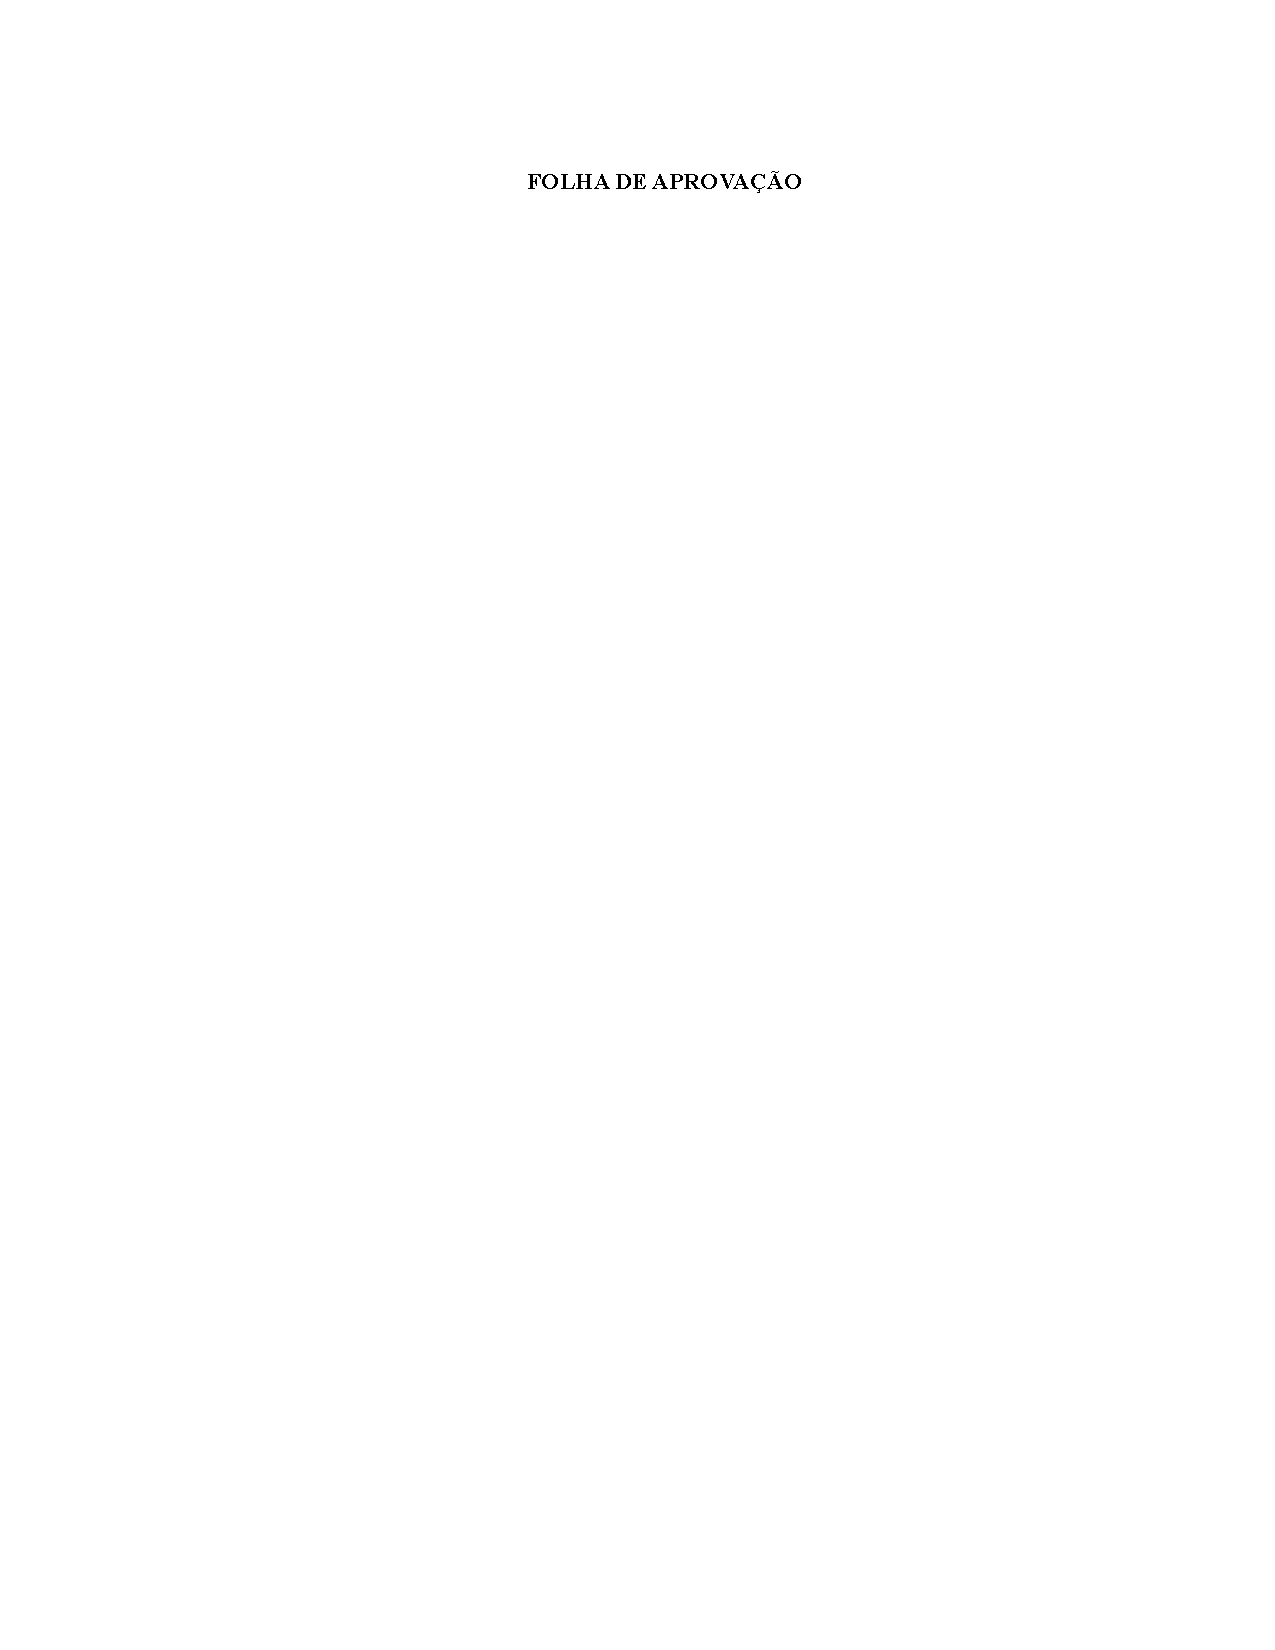
\includepdf[scale=1.0,pages=1]{./PreTexto/folha-aprovacao.pdf} % para adicionar o pdf enviado pelo professor apenas substitua o documento folha-aprovacao.pdf dentro da pasta PreTexto

%% Dedicatória
%%%% DEDICATÓRIA
%%
%% Texto em que o autor presta homenagem ou dedica seu trabalho.

\begin{dedicatoria}%% Ambiente dedicatoria

%Espaço destinado à dedicatória (elemento opcional). Folha que contém o oferecimento do trabalho à determinada pessoa ou pessoas. Exemplo:



Dedico este trabalho à minha família, pelos momentos de ausência.

\end{dedicatoria}
%% Comente para remover este item

%% Agradecimentos
\begin{agradecimentos}%% Ambiente agradecimentos
    Primeiramente, agradeço a minha família, em especial ao meu pai e minha mãe, que foram meu grande apoio ao longo de toda essa jornada, sem os seus ensinamentos e apoio nada disso seria possível.

    Agradeço aos meus orientadores Prof. Dr. João Fabrício Filho e ao Prof. Dr. Rogério Aparecido Gonçalves, pelas suas orientações e contribuições valiosas, não só neste trabalho como também ao longo de toda minha Iniciação Científica.

    Também agradeço a minha namorada pela sua companhia e estar ao meu lado nos momentos dificéis.

    Enfim, agradeço a todos que direta ou indiretamente me ajudaram e estiveram no meu lado durante minha caminhada.
\end{agradecimentos}
%% Comente para remover este item

%% Epígrafe
%%%% EPÍGRAFE
%%
%% Texto em que o autor apresenta uma citação, seguida de indicação de autoria, relacionada com a matéria tratada no corpo do
%% trabalho.

\begin{epigrafe}%% Ambiente epigrafe
%
%Espaço destinado à epígrafe (elemento opcional). Nesta folha, o(a) autor(a) usa uma citação, seguida de indicação de autoria e ano, relacionada, preferencialmente, com o assunto tratado no corpo do trabalho. A citação deverá constar na lista de referências. Exemplo: 
%
``A biblioteca é um jardim onde as ideias florescem e os frutos são colhidos pela eternidade.'' \cite{Candido2002}.
\end{epigrafe}
%% Comente para remover este item

%% Resumo
\begin{resumoutfpr}
    Com o fim da Lei de Moore e da escala de Dennard, diferentes técnicas computacionais surgiram para suprir a demanda por maior desempenho computacional e eficiência energética. A Computação Aproximada é um paradigma que visa aumentar o desempenho e a eficiência energética de aplicações em troca de pequenas perdas de precisão. A Computação Paralela também surge como um paradigma de computação que busca obter maior desempenho por meio de um melhor aproveitamento dos processadores \textit{multicore}. O \texttt{OpenMP} surge como uma ferramenta desse paradigma, facilitando o desenvolvimento de aplicações paralelas por meio de anotações de código. A proposta deste trabalho é implementar diferentes técnicas de aproximação no \texttt{OpenMP} por meio de modificações em sua infraestrutura no LLVM. As técnicas propostas são: perfuração de laços, memoização aproximada, descarte de tarefas e relaxamento de ponto flutuante. As técnicas propostas foram avaliadas utilizando um \textit{benchmark suite} composto pelas aplicações \textit{K-Means}, \textit{2MM}, \textit{Correlação}, \textit{Deriche}, \textit{Jacobi 2D}, \textit{Mandelbrot} e \textit{PI de Monte Carlo}.
\end{resumoutfpr}

%De acordo com a NBR 6028:2021, a apresentação gráfica deve seguir o padrão do documento no qual o resumo está inserido. Para definição das palavras-chave (e suas correspondentes em inglês no abstract) consultar em Termo tópico do Catálogo de Autoridades da Biblioteca Nacional, disponível em: http://acervo.bn.gov.br/sophia_web/autoridade%% Comente para remover este item

%% Abstract
%%%% ABSTRACT
%%
%% Versão do resumo para idioma de divulgação internacional.

\begin{abstractutfpr}%% Ambiente abstractutfpr
Seguir o mesmo padrão do resumo, com a tradução do texto do resumo e referência, se houver, para a língua estrangeira (língua inglesa).
\end{abstractutfpr}
%% Comente para remover este item

%% Lista de algoritmos
%\incluirlistadealgoritmos%% Comente para remover este item


%% Lista de Ilustrações
%% Figuras, Gráficos, Quadros e Fotografias são incluídos juntos em uma mesma lista
%% Na UTFPR sugere-se adotar listas próprias, conforme a natureza da ilustração, a partir da existência de 3 elementos da mesma natureza.Neste caso, cada lista deverá iniciar em folha distinta. Não criar listas com apenas um item.


\incluirlistadeilustracoes


%% Lista de figuras
%\incluirlistadefiguras%% Comente para remover este item

%\incluirlistageraldeilustracoes
%\listofgeneralilust



%% Lista de Fotografias
%\incluirlistadefotografias %% Comente para remover este item


%% Lista de Gráficos
%\incluirlistadegraficos %% Comente para remover este item

%% Lista de tabelas
\incluirlistadetabelas%% Comente para remover este item

%% Lista de quadros
%\incluirlistadequadros

%% Listagem de códigos fonte
%\incluirlistadecodigosfonte

%% Lista de abreviaturas, siglas e acrônimos
\incluirlistadeacronimos{glossaries}%% Opções: "glossaries" (pacote) ou "file" (arquivo) ou "none" (desabilita)

%% Lista de símbolos
% \incluirlistadesimbolos{file}%% Opções: "nomencl" (pacote) ou "file" (arquivo) ou "none" (desabilita)

%% Sumário
\incluirsumario%% Comente para remover este item

%% Formatação de páginas de elementos textuais
\textual%% Não comente esta linha

%% Parte
% \part{Introdução}%% Comente para remover este item

%% Capítulos

\chapter{Introdução}\label{cap:introducao}

Por décadas, a Lei de Moore e a escala de Dennard impulsionaram melhorias exponenciais no desempenho computacional e na eficiência energética. A Lei de Moore possibilitou maiores densidades de transistores, enquanto a escala de Dennard garantiu que o consumo de energia permanecesse controlado. À medida que a tecnologia se aproximou de limites fundamentais, ambas as tendências entraram em colapso, tornando os ganhos de desempenho cada vez mais difíceis, hoje limitados a apenas alguns poucos por cento ao ano~\cite{hennessy2019}. Mesmo com essas limitações, a crescente demanda por maior desempenho computacional e eficiência energética tem impulsionado inovações em uma ampla variedade de plataformas, desde sistemas embarcados até \textit{datacenters}. Essa demanda é impulsionada pela crescente complexidade das cargas de trabalho modernas, como análise de dados em tempo real, aprendizado de máquina e processamento de sinais, que frequentemente exigem vastos recursos computacionais~\cite{mittal2016, dalloo2024}.

Para atender a essas demandas sob restrições de desempenho e energia, pesquisadores têm explorado paradigmas alternativos de computação. A \gls{ca} é um paradigma que busca equilibrar precisão computacional e eficiência de recursos. Ela parte do princípio de que muitas aplicações não necessitam de resultados exatos, mas sim de resultados suficientemente precisos dentro de limites aceitáveis, definidos pela percepção do usuário ou por métricas de qualidade específicas~\cite{dalloo2024}. Ao explorar a diferença entre a precisão realmente exigida e a tradicionalmente garantida pelos sistemas, a \gls{ca} viabiliza ganhos expressivos em desempenho, consumo de energia e utilização de \textit{hardware}~\cite{xu2016,leon2025a,leon2025b}.

A \gls{cp} é outro paradigma amplamente adotado nos últimos anos, especialmente com a popularização de processadores \textit{multicore} em computadores pessoais e dispositivos móveis. Essa tendência intensificou a necessidade de desenvolver softwares paralelos, estimulando o surgimento de ferramentas que simplificam a criação dessas aplicações~\cite{goncalves2016}. O \texttt{OpenMP} é uma dessas ferramentas: ele permite que desenvolvedores anotem o código para execução paralela, delegando ao compilador a maior parte da complexidade de gerenciamento~\cite{alrawais2021}. Esse paradigma tornou-se essencial em \gls{hpc}, especialmente em simulações científicas, que tipicamente demandam elevado poder de processamento~\cite{adhikari2012}.

Embora as técnicas de \gls{ca} ofereçam benefícios expressivos, sua aplicação eficaz requer a identificação cuidadosa de regiões de código onde a aproximação seja segura e vantajosa. Esse processo normalmente exige análise detalhada do comportamento da aplicação e de seus requisitos de qualidade~\cite{sampson2015,reis2021}. Este trabalho parte da hipótese de que é possível melhorar o desempenho de aplicações combinando técnicas de aproximação e paralelização, preservando a facilidade de uso provida por ferramentas como o \texttt{OpenMP}. Dessa forma, busca-se explorar simultaneamente os ganhos oferecidos pela execução paralela e pela computação aproximada.

\section{Objetivos}\label{cap:objetivos}

O objetivo geral deste trabalho é melhorar o desempenho de aplicações de \gls{hpc} por meio da aplicação combinada de técnicas de aproximação e paralelização.

Para atingir esse objetivo, foram definidos os seguintes objetivos específicos:
\begin{itemize}
    \item Desenvolver um \textit{benchmark} voltado à avaliação de técnicas de \gls{ca};
    \item Implementar uma extensão do \texttt{OpenMP} com suporte a técnicas de aproximação baseadas em anotações;
    \item Adicionar suporte em tempo de execução para múltiplos algoritmos de aproximação dentro do \texttt{runtime} do \texttt{OpenMP};
    \item Integrar um passo de perfuração de laços ao pipeline de otimização do LLVM;
    \item Realizar a avaliação experimental das técnicas propostas em um ambiente de \gls{ca}.
\end{itemize}

\section{Contribuições}\label{cap:contribuicoes}

As principais contribuições deste trabalho são: o desenvolvimento de um \textit{benchmark suite} voltado à avaliação de \gls{ca}, a implementação de uma extensão do \texttt{OpenMP} com suporte a técnicas de aproximação e a integração dessas funcionalidades à infraestrutura do LLVM. As aplicações que compõem o \textit{benchmark} foram selecionadas com base em conjuntos amplamente utilizados, como o PolyBench~\cite{polybench} e o Debian Benchmarks Game~\cite{debianBenchmarksGame}, e adaptadas para suportar anotações com \texttt{OpenMP}. Também foi implementada uma infraestrutura para avaliação da aceitabilidade dos resultados produzidos. A extensão proposta exigiu modificações na infraestrutura do LLVM, bem como adaptações em algoritmos e escalonadores do \texttt{OpenMP}, a fim de possibilitar o suporte a tarefas aproximadas.

\section{Organização do Trabalho}\label{cap:org_trabalho}

O restante deste trabalho está organizado da seguinte forma: no \autoref{cap:fundamentacaoTeorica} são apresentados os conceitos fundamentais de \gls{ca} e \gls{cp} relacionados a este estudo, incluindo as técnicas de aproximação abordadas — perfuração de laço, memoização aproximada, descarte de tarefas e relaxamento de ponto flutuante, além de uma introdução ao \texttt{OpenMP} e uma revisão de trabalhos correlatos. No \autoref{cap:proposta} é apresentada a proposta dos construtores implementados no \texttt{OpenMP} utilizando a infraestrutura do LLVM. No \autoref{cap:metodologia} são detalhadas a metodologia e as ferramentas empregadas para a realização dos experimentos. Por fim, o \autoref{cap:cronograma} apresenta o cronograma de execução deste trabalho.



\chapter{Fundamentaç\~ao Te\'orica}\label{cap:fundamentacaoTeorica}

Este capítulo apresenta os conceitos relacionados a \gls{ca} e Computação Paralela. Primeiramente aborda-se a definição de \gls{ca}, seu uso em aplicações, os desafios enfrentados por essa estratégia e o detalhamento dos algoritmos de perforação de laço, memoização, aproximação de ponto flutuante e o descarte de tarefas. Por fim apresenta também conceitos de Computação Paralela com um foco no uso da ferramenta OpenMP.

\section{Computação aproximada}\label{sec:compAprox}

A \gls{ca} consiste em um conjunto de técnicas aplicadas a cenários em que os resultados exatos não são estritamente necessários ou em que as aplicações apresentam resiliência suficiente para lidar com pequenas imprecisões em suas computações. Nessas situações, o uso de tais técnicas pode proporcionar ganhos significativos de desempenho e eficiência energética, mantendo a margem de erro em níveis reduzidos. Um exemplo é o uso de redes neurais para aproximar a divergência de \textit{branch} em instruções \gls{simd}, capaz de alcançar aceleração de até 14,8$\times$ com acurácia de 96\%~\cite{grigorian2015}. Por esse motivo, a \gls{ca} se mostra especialmente atraente em domínios como análise de dados, reconhecimento de padrões, processamento de imagens e sinais~\cite{mittal2016, chippa2013}.

As diferentes estratégias de aproximação podem ser classificadas conforme a camada em que são aplicadas na pilha computacional. No nível de \textit{hardware}, destacam-se técnicas que envolvem desde unidades funcionais aproximadas, como somadores, multiplicadores e divisores, até abordagens como \textit{overclocking}~\cite{leon2025a,leon2025b} e o uso de memórias aproximadas~\cite{fabricio2020}. No nível de \textit{software}, encontram-se estratégias mais generalistas, incluindo linguagens de programação aproximada~\cite{sampson2015}, \textit{runtimes} com suporte à aproximação~\cite{li2018,reis2024} e otimizações realizadas em nível de compilador~\cite{oliveira2024a,oliveira2024b}.

Apesar de seus benefícios, esse paradigma enfrenta desafios significativos. Em primeiro lugar, nem todas as aplicações são resilientes a erros em sua execução, o que limita o uso de técnicas mais generalistas e torna necessário definir métricas que permitam ajustar o grau de precisão desejado, seja pelo usuário ou pela própria aplicação~\cite{mittal2016}. Além disso, medir corretamente o nível de erro introduzido não é trivial, pois nem sempre está claro qual métrica deve ser aplicada à saída da aplicação~\cite{felzmann2021}. Outro ponto crítico é a propagação dos erros, que pode comprometer toda a execução: em alguns casos, a aplicação pode falhar abruptamente; em outros, concluir sua execução de forma aparentemente correta, mas com resultados significativamente distantes do esperado~\cite{fabricio2020}.

Diante disso é possível observar que a \gls{ca} não se restringe a um único método, mas a um conjunto de diversas estratégias que exploram diferentes aspectos da execução de um programa. Na subseção seguinte, são detalhados quatro dessas estratégias: perforação de laço, memoização, aproximação de ponto flutuante e o descarte de tarefas

\subsection{Perforação de laço}\label{subsec:perfLaco}

A perforação de laço é uma das técnicas mais simples de computação aproximada, cuja ideia central consiste em omitir determinadas iterações de um laço, reduzindo assim o tempo de execução de uma região de código~\cite{sidiroglou2011}.

Existem diferentes forma de implementar esse técnica, existem técnicas estáticas que são aplicadas em tempo de compilação e outras dinâmicas que permitem ajustar o grau de omissão em tempo de execução~\cite{li2018}.

Em ambos os casos é comum implementar essa otimização em laços que estão em um formato canônico~\cite{openmp2018}. A \autoref{code:loopCanon} apresenta a estrutura de um laço canônico, geralmente expresso na forma de um \texttt{for}, com três elementos principais:

\begin{itemize}
    \item \textbf{Expressão inicial:} define o limite inferior do laço, ou seja, o ponto em que a computação começa.
    \item \textbf{Expressão de teste:} geralmente um operador relacional que compara a variável de indução com o limite superior, delimitando o espaço de iterações.
    \item \textbf{Expressão de incremento/decremento:} atualiza a variável de indução e define o passo do laço.
\end{itemize}

\begin{sourcecode}[htb]\caption{\label{code:loopCanon}Estrutura de um laço canônico}
    \begin{lstlisting}[frame=single, language=C++]
        for (int i = 0; i < N; i += a) {
            ...
        }
    \end{lstlisting}
    \fonte{}
\end{sourcecode}

Uma técnica comumente encontrada na implementação desse algoritmo é a de incrementar a expressão de incremento, se considerarmos isso no \autoref{code:loopCanon} teríamos que a iterações deixariam de ser de \texttt{a} em \texttt{a} vezes, passaríamos a ter um incremento de \texttt{a + 1} vezes. Se considerarmos que inicialmente tem o valor \texttt{a = 1} ele passaria a ser \texttt{a = 2} e o comportamento do laço seguiria o que está na \autoref{fig:perfoMod}, nela temos que os blocos em branco seriam iterações não executadas enquanto os blocos em azul seriam iterações executadas.

Uma forma simples de aplicar a perforação de laço é alterar o passo do incremento da variável de indução, de modo que parte das iterações seja ignorada. No exemplo da \autoref{code:loopCanon}, se inicialmente o incremento for \texttt{a = 1} (\texttt{i++}), todas as iterações serão executadas. Entretanto, ao modificar o incremento para \texttt{a = 2} (\texttt{i += 2}), apenas metade delas será realizada, já que o laço passa a “pular” uma iteração a cada passo. Esse comportamento é ilustrado na \autoref{fig:perfoMod}, onde blocos em azul representam iterações executadas e blocos em branco representam iterações omitidas.

\begin{figure}[htb]
    \caption{Modelo de execução do algoritmo de perforação de laço}
    \label{fig:perfoMod}
    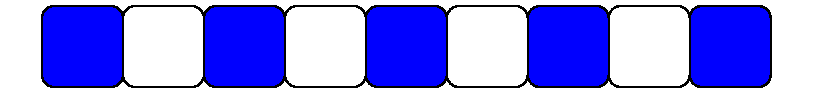
\includegraphics[scale=0.7]{figuras/loop_perfo.pdf}
    \fonte{}
    \addcontentsline{loge}{figure}{\protect\numberline{\thefigure}Modelo de execução do algoritmo de perforação de laço.}
\end{figure}

\subsection{Memoização}\label{subsec:memo}

A memoização é tradicionalmente uma técnica associada à programação dinâmica que utiliza uma \textit{cache} de resultados para acelerar a execução de determinadas computações. Seu princípio consiste em armazenar os resultados de chamadas já realizadas, indexados pelas entradas correspondentes. Assim, quando a função é invocada novamente com os mesmos parâmetros, o valor previamente calculado é retornado diretamente, evitando a repetição da computação~\cite{michie1968}.

A memoização aproximada, também chamada de memoização temporal, estende esse conceito ao considerar tempo de execução e localização como critérios adicionais. Sua ideia principal é explorar o fato de que chamadas consecutivas a uma mesma função tendem a produzir resultados similares~\cite{tziantzioulis2018}.

Na prática, as saídas são armazenadas em uma estrutura de dados e reutilizadas seletivamente em chamadas subsequentes. As estratégias de \textit{cache} podem variar, incluindo modelos globais, específicos por função ou mesmo dependentes de contexto. O reuso é normalmente controlado por um limiar de tolerância, que avalia a variação das saídas: se os resultados permanecerem estáveis dentro desse limite, a função é considerada estável e, portanto, pode ser memoizada~\cite{tziantzioulis2018}.

\subsection{Aproximação de ponto flutuante}\label{subsec:pontoFlut}

A representação de números reais por meio de números de ponto flutuante envolvem aproximação por padrão devido a impossibilidade de representar valores contínuos, se torna impossível representar um número infinito com um número finito de \textit{bits}~\cite{monniaux2008}. Por esse motivo aritmética com números de ponto flutuante usualmente introduzem erros de aproximação que variam conforme a ordem de execução dessas operações, resultando em um valor completamente diferente do esperado. Um exemplo disso pode ser obervado na \autoref{fig:floatPoint}.

\begin{figure}[htb]
    \caption{Erro introduzido na aritmética de ponto flutuante.}
    \label{fig:floatPoint}
    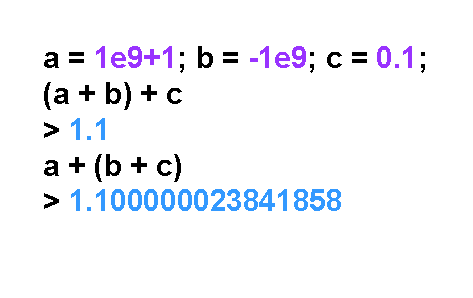
\includegraphics[scale=0.7]{figuras/fastmath.pdf}
    \fonte{}
    \addcontentsline{loge}{figure}{\protect\numberline{\thefigure}Erro introduzido na aritmética de ponto flutuante.}
\end{figure}

Para reduzir este tipo de problema, compiladores usualmente evitam aplicar certas otimizações que podem amplificar o erro nesse tipo de operação. Porém, alguns compiladores como é o caso do \texttt{Clang} e o \texttt{GCC}, suportam a opção \texttt{--fast-math} que passa a permitir a aplicação dessas otimizações em todo um módulo de compilação~\cite{gccffast, clangffast}. E de maneira similar o \texttt{MSVC} suporta o uso da diretiva de compilação \texttt{\#pragma float\_control} para definir regiões do código que permitem o uso dessas otimizações em certas regiões decódigo~\cite{msvcfast}.

\subsection{Descarte de tarefas}\label{subsec:descTar}

O descarte de tarefas é um conceito abrangente que engloba diferentes técnicas de aproximação, incluindo, em alguns casos, a própria perforação de laço. Sua ideia central baseia-se em computações que podem ser divididas em unidades menores, chamadas tarefas, das quais uma parte delas é descartada~\cite{mittal2016}.

As implementações dessa técnica costumam adotar uma taxa de descarte, que define a fração de tarefas a serem eliminadas durante a execução do programa. A \autoref{fig:perfoMod} também pode ser utilizada para ilustrar esse mecanismo: os blocos brancos representam tarefas descartadas, enquanto os blocos azuis indicam as tarefas efetivamente executadas.

\section{Computação paralela}\label{sec:compParalela}

A \gls{cp} é uma área da computação que busca explorar arquiteturas modernas, cada vez mais baseadas em processadores \textit{multicore}. Esse conceito pode ser melhor compreendido a partir da taxonomia de Flynn~\cite{flynn1972}, que classifica as arquiteturas de computadores de acordo com o fluxo de instruções e de dados:

\begin{itemize}
    \item \textbf{SISD (\textit{Single Instruction, Single Data stream}):} Instrução única que atua sobre uma única fonte de dados.
    \item \textbf{SIMD (\textit{Single Instruction, Multiple Data stream}):} Instrução única que é aplicada simultaneamente a múltiplos dados.
    \item \textbf{MISD (\textit{Multiple Instructions, Single Data stream}):} Múltiplas instruções atuando sobre uma mesma fonte de dados.
    \item \textbf{MIMD (\textit{Multiple Instructions, Multiple Data stream}):} Múltiplas instruções atuando em paralelo sobre múltiplas fontes de dados.
\end{itemize}

Dentro desse modelo, o paralelismo pode ser explorado de diferentes maneiras. No nível do processador, técnicas como \textit{pipeline}, predição de desvios (\textit{branch prediction}) e escalonamento dinâmico permitem dividir o código em pequenas unidades que podem ser executadas simultaneamente.

Algumas arquiteturas foram além e incorporaram extensões \gls{simd}, permitindo a utilização de processadores vetoriais capazes de realizar a mesma operação sobre múltiplos elementos de um vetor unidimensional em um único ciclo de instrução. Em cenários mais especializados, como nas \glspl{gpu}, esse modelo é expandido para múltiplas dimensões de dados, possibilitando que milhares de operações sejam executadas em paralelo e tornando-as altamente adequadas para cargas de trabalho massivamente paralelizáveis~\cite{hennessy2017}. Outro mecanismo fundamental é o uso de \textit{threads}, que representam abstrações de execução em nível de software, permitindo que diferentes unidades computacionais operem concorrentemente em múltiplos processadores. Cada \textit{thread} possui seu próprio contexto de execução, mas pode compartilhar recursos como memória e dispositivos de entrada/saída, viabilizando desde o paralelismo de tarefas independentes até a cooperação em algoritmos que exploram granularidades mais finas~\cite{tanenbaum2015,hennessy2017}.

É nesse contexto que surge o OpenMP, uma \gls{api} projetada para estender C, C++ e Fortran com suporte à paralelização de aplicações por meio de anotações de código. Essas anotações especificam o como aquela região de código deve ser executada. Seu modelo de programação permite explorar automaticamente diferentes formas de paralelismo, seja pelo \textit{offloading} para \glspl{gpu}, pelo uso de múltiplas \textit{threads}, ou ainda pela vetorização via \gls{simd}, aproveitando as unidades vetoriais das arquiteturas modernas~\cite{mattson2019}.

\begin{figure}[htb]
    \caption{Arquitetura do \texttt{OpenMP}.}
    \label{fig:ompArchitecture}
    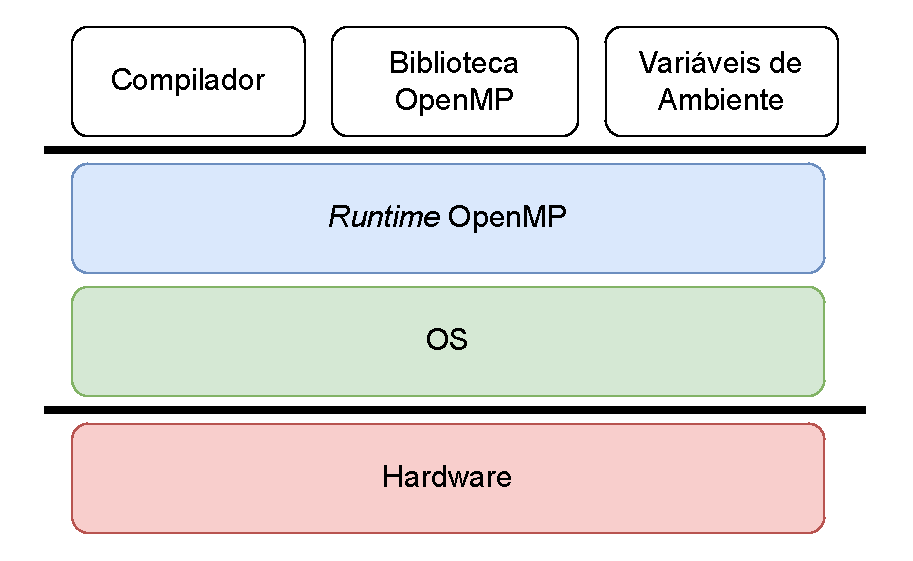
\includegraphics[scale=0.7]{figuras/omp_architecture.pdf}
    \fonte{}
    \addcontentsline{loge}{figure}{\protect\numberline{\thefigure}Arquitetura do \texttt{OpenMP}.}
\end{figure}

O OpenMP é estruturado em uma arquitetura em camadas, composta por anotações de código, suporte da \textit{runtime} e configurações do ambiente de execução, conforme ilustrado na FIGURA. Esse modelo permite ao programador controlar diversos aspectos da execução por meio de diretivas e chamadas à biblioteca, como a definição do número de \textit{threads} em uma região paralela e a escolha do comportamento do escalonador. Dessa forma, o OpenMP oferece um controle flexível sobre o paralelismo do programa.

A \autoref{code:produtoVet} apresenta a implementação sequencial de um produto escalar entre vetores. A paralelização utilizando a biblioteca \texttt{pthreads}, apresentada no \autoref{code:produtoThread}, exige a criação explícita de \textit{threads}, gerenciamento de regiões de memória e sincronização dos resultados parciais. Em contraste, o \autoref{code:produtoOmp} implementado com o OpenMP, evidencia a simplicidade proporcionada pelas diretivas: uma única anotação é suficiente para paralelizar o laço de cálculo, delegando à \textit{runtime} a criação e sincronização das \textit{threads}.

\begin{sourcecode}[htb]\caption{\label{code:produtoVet}Estrutura de um laço canônico}
    \begin{lstlisting}[frame=single, language=C++]
        for (int i = 0; i < N; i++) {
            result += a[i] * b[i];
        }
    \end{lstlisting}
    \fonte{}
\end{sourcecode}

\begin{sourcecode}[htb]\caption{\label{code:produtoThread}Estrutura de um laço canônico}
    \begin{lstlisting}[frame=single, language=C++]
        void *compute_partial_dot(void *arg) {
            ThreadArgs *args = (ThreadArgs *)arg;
            args->partial_sum = 0.0;
            
            for (int i = args->start; i < args->end; i++) {
                args->partial_sum = 0.0; += args->a[i] * args->b[i];
            }

            return NULL;
        }

    ...

    pthread_t threads[NUM_THREADS];
    ThreadArgs args[NUM_THREADS];
    result = 0.0;
    chunk_size = N / NUM_THREADS;

    for (int i = 0; i < NUM_THREADS; i++) {
        args[i].start = i * chunk_size;
        args[i].end = (i == NUM_THREADS - 1) ? N : (i + 1) * chunk_size;
        args[i].a = a;
        args[i].b = b;
        pthread_create(&threads[i], NULL, compute_partial_dot, &args[i]);
    }

    for (int i = 0; i < NUM_THREADS; i++) {
        pthread_join(threads[i], NULL);
        result += args[i].partial_sum;    
    }
    \end{lstlisting}
    \fonte{}
\end{sourcecode}

\begin{sourcecode}[htb]\caption{\label{code:produtoOmp}Estrutura de um laço canônico}
    \begin{lstlisting}[frame=single, language=C++]
        #pragma omp parallel for reduction(+ : result)
        for (int i = 0; i < N; i++) {
            result += a[i] * b[i];
        }
    \end{lstlisting}
    \fonte{}
\end{sourcecode}

Tipicamente, uma diretiva OpenMP é aplicada a um laço para indicar que ele pode ser executado em paralelo. Durante a compilação, esse bloco de código é isolado e transformado em tarefas, enquanto a \textit{runtime} prepara as estruturas necessárias para o modelo \textit{fork-join}. Por exemplo, a diretiva \texttt{\#pragma omp parallel} cria um time de \textit{threads}, cada uma executando uma cópia do código anotado. O compilador gerencia variáveis privadas, memória de pilha e pontos de sincronização automaticamente. Ao final, as \textit{threads} são reunificadas (\textit{joined}), e a execução retorna ao fluxo sequencial. Essa abordagem permite paralelizar regiões de código com esforço reduzido de gerenciamento, mantendo controle sobre sincronização e compartilhamento de dados~\cite{mattson2019}.

\begin{figure}[htb]
    \caption{Modelo \textit{fork-join} de execução do \texttt{OpenMP}.}
    \label{fig:ompExec}
    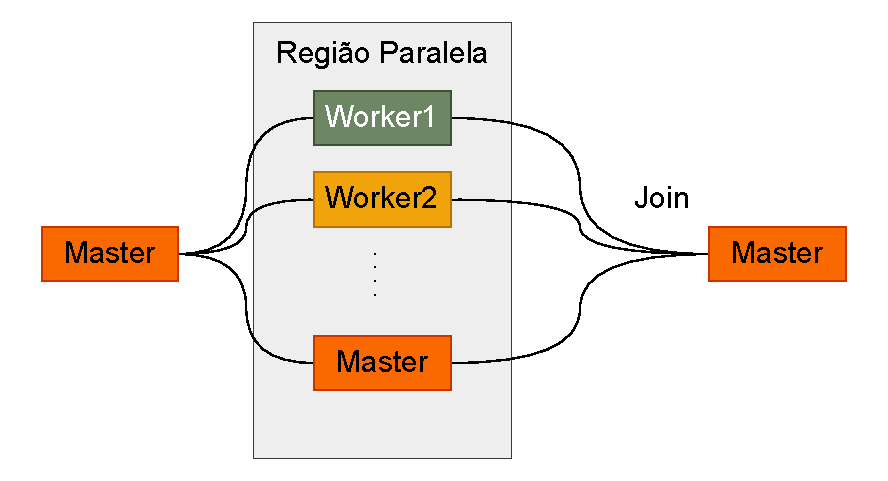
\includegraphics[scale=0.7]{figuras/omp_exec.pdf}
    \fonte{}
    \addcontentsline{loge}{figure}{\protect\numberline{\thefigure}Modelo \textit{fork-join} de execução do \texttt{OpenMP}.}
\end{figure}

O modelo \textit{fork-join} pode ser observado de forma esquemática na \autoref{fig:ompExec}. Nele, a \textit{runtime} cria múltiplas \textit{threads} para a execução paralela, que são sincronizadas ao final, restando apenas a \textit{thread} principal para continuar a execução sequencial. O OpenMP também suporta regiões paralelas aninhadas, possibilitando hierarquias de paralelismo.

\section{Trabalhos Relacionados}\label{sec:trabRelac}

Esta seção apresenta arcabouços baseados no paradigma de \gls{ca} que implementam suporte em nível de linguagem de programação, especialmente aqueles que utilizam anotações de código e mecanismos de execução em \textit{runtime}. Os arcabouços e aplicações selecionados buscam oferecer ao desenvolvedor maior controle sobre as técnicas utilizadas e sobre as regiões de código que podem ser aproximadas.

O ACCEPT~\cite{sampson2015} (Approximate C Compiler for Energy and Performance Trade-Off) é um arcabouço implementado sobre a infraestrutura do LLVM, que introduz a palavra-chave \texttt{ACCEPT} na sintaxe das linguagens C/C++. Essa palavra-chave permite diferenciar regiões de código aproximadas daquelas que devem ser executadas de forma precisa. O arcabouço também implementa etapas de análise para verificar a possibilidade de aproximação dessas regiões, avaliando não apenas a validade das transformações, mas também viabilizando a aplicação de diferentes técnicas de otimização aproximada, de maneira análoga ao funcionamento de um compilador paralelizador.

A infraestrutura do ACCEPT permite, por meio de anotações de código e análises estáticas e dinâmicas, identificar regiões de código potencialmente aproximáveis. Essas regiões podem ser exploradas para aplicar técnicas como perforação de laço, elisão de sincronização e até mesmo o uso de redes neurais em \textit{hardware} para estimar saídas. Além disso, o arcabouço incorpora um \textit{autotuner} que utiliza métricas fornecidas pelo usuário para avaliar se as aproximações aplicadas mantêm a qualidade de saída dentro dos limites esperados, garantindo que o programa não apresente falhas durante a execução.

Vassiliadis et al.~\cite{vassiliadis2015} propõem uma extensão ao OpenMP que incorpora suporte à \gls{ca} no modelo de programação baseado em tarefas. Em sua proposta, o programador pode especificar funções aproximadas alternativas que podem ser escolhidas em tempo de execução para substituir versões precisas de determinadas tarefas. Assim, parte das tarefas é executada de forma exata, enquanto outras utilizam versões aproximadas, reduzindo o consumo energético e mantendo a qualidade de acordo com limites definidos pelo usuário.

O arcabouço também introduz um mecanismo de barreira para garantir que uma fração mínima das execuções alcance o grau de acurácia desejado. Para gerenciar essa execução, são propostas duas políticas no runtime: \textit{Global Task Buffering} (GTB), que toma decisões informadas a partir da análise conjunta de todas tarefas pendentes, e a \textit{Local Queue History} (LQH), baseada no histórico local de filas, em que cada \textit{worker} decide de maneira autônoma o nível de aproximação com base nas execuções anteriores.

Lashgar et al.~\cite{lashgar2018} propõem a integração da técnica de perforação de laço ao \texttt{OpenACC} com o objetivo de melhorar o desempenho, executando apenas um subconjunto das iterações do laço. Dessa forma, parte das saídas é calculada de maneira exata, enquanto o restante é aproximado. Para mitigar os impactos dessa abordagem na precisão e no tempo de execução dentro do \texttt{OpenACC}, os autores introduzem um mecanismo de correção implementado diretamente no kernel. Esse mecanismo identifica as saídas ausentes e aplica estratégias como a cópia ou a média dos valores vizinhos já computados, a fim de estimar as entradas faltantes.

O HPAC~\cite{parasyris2021} é um arcabouço de técnicas de computação aproximada voltadas para aplicações HPC, implementado sobre a infraestrutura do LLVM. Ele utiliza anotações de código \texttt{pragma} para C/C++, permitindo a definição de regiões de código aproximadas, e se destaca por sua interoperabilidade com o OpenMP. As técnicas principais incluem perforação de laço e memoização aproximada, e o arcabouço fornece ainda uma ferramenta de análise que permite ao usuário anotar múltiplas regiões de código e avaliar a qualidade dos resultados obtidos para cada configuração.

O HPAC-Offload~\cite{fink2023} é uma extensão do HPAC~\cite{parasyris2021} voltada para aplicações em GPU, que adapta sua arquitetura para lidar com as limitações do modelo de memória e paralelismo dessas plataformas. Assim como no HPAC, as técnicas implementadas incluem perforação de laço e memoização aproximada, mas com um gerenciamento de memória consciente da GPU: os dados internos de AC são armazenados na memória compartilhada do bloco, permitindo reutilização entre threads ativas sem sobrecarregar a memória global. O arcabouço também define níveis hierárquicos de aproximação (\textit{thread}, \textit{warp} e bloco) para evitar divergência e deadlocks.

Em contraste com outros trabalhos, nossa abordagem baseia-se na extensão do próprio framework \texttt{OpenMP}, modificando sua \textit{runtime} e alterando suas diretivas de compilação para oferecer suporte nativo a técnicas de \gls{ca}. Ao incorporar o controle de aproximação diretamente no \texttt{OpenMP}, habilitamos o escalonamento e a execução de tarefas sem comprometer sua API. Essa integração não apenas simplifica a adoção de \gls{ca} em computação paralela, como também abre caminho para uma exploração mais ampla e eficaz da aproximação em aplicações que já utilizam o OpenMP. A Tabela~\ref{tab:trabComp}, apresenta um breve resumo e comparação entre todos os trabalhos citados.

\begin{table}[htb]
    \centering
    \caption{Resumo e comparação entre os trabalhos citados}
    \begin{tabular}{|p{2.3cm}|p{3cm}|p{2cm}|p{3cm}|p{4cm}|}
        \hline
        \textbf{Trabalho}                         & \textbf{Linguagem / Infraestrutura} & \textbf{Suporte a Paralelismo} & \textbf{Técnicas de Aproximação}                                                                        & \textbf{Diferenciais}                                                                                                                                                      \\
        \hline
        ACCEPT~\cite{sampson2015}                 & C/C++, LLVM                         & Sequencial e paralelo          & Perforação de laço, elisão de sincronização e redes neurais em \textit{hardware}                        & Validação de aproximações em tempo de execução; Aplicação de múltiplas técnicas de otimização                                                                              \\
        \hline
        Vassiliadis et al.~\cite{vassiliadis2015} & C/C++, OpenMP                       & Paralelismo baseado em tarefas & Funções aproximadas                                                                                     & Controle de acurácia; Decisões globais e locais para aproximação                                                                                                           \\
        \hline
        Lashgar et al.~\cite{lashgar2018}         & C/C++, OpenACC                      & Paralelismo em laço            & Perforação de laço                                                                                      & Estima valores ausentes para manter precisão em laços aproximados                                                                                                          \\
        \hline
        HPAC~\cite{parasyris2021}                 & C/C++, LLVM, OpenMP                 & Regiões paralelas              & Perforação de laço, memoização aproximada                                                               & Interoperabilidade com OpenMP; Análise de múltiplas regiões de código                                                                                                      \\
        \hline
        HPAC-Offload~\cite{fink2023}              & C/C++, LLVM, OpenMP                 & Paralelismo via GPU            & Perforação de laço, memoização aproximada                                                               & Interoperabilidade com OpenMP; Hierarquia de aproximação em GPU                                                                                                            \\
        \hline
        \textbf{Este Trabalho}                    & \textbf{C/C++, LLVM, OpenMP}        & \textbf{Regiões paralelas}     & \textbf{Perforação de laço, memoização aproximada, aproximação em ponto flutuante, descarte de tarefas} & \textbf{Integração direta com OpenMP; Combina análise em tempo de compilação e decisões em tempo de execução; Aplica múltiplas técnicas de aproximação visando desempenho} \\
        \hline
    \end{tabular}
    \fonte{}
    \label{tab:trabComp}
\end{table}


\chapter{Proposta}\label{cap:proposta}

Este trabalho apresenta um novo construtor para o \texttt{OpenMP} que facilita a implementação de algoritmos de aproximação. Assim como outros construtores da API, a proposta utiliza anotações de código — os \texttt{pragma} em C/C++ — para identificar regiões que podem ser executadas de forma aproximada. A integração dessas anotações ao arcabouço do \texttt{OpenMP} assegura que as técnicas sejam portáteis e facilmente adaptáveis a diferentes trechos de código.

O \autoref{code:pragmaApprox} apresenta a anotação \texttt{pragma approx}, que delimita uma região de código a ser aproximada e especifica a técnica a ser aplicada. Múltiplas cláusulas podem ser combinadas em um único construtor para indicar diferentes parâmetros de aproximação. Entretanto, a implementação atual suporta apenas uma técnica de aproximação

\begin{sourcecode}[htb]\caption{\label{code:pragmaApprox}Sintaxe do construtor \texttt{approx}}
    \begin{lstlisting}[frame=single, language=C++]
        #pragma omp approx [clause, [[,]clause]]
    \end{lstlisting}
    \fonte{}
\end{sourcecode}

\section{Perforação de laço}\label{subsec:pragmaPerfo}

A cláusula \texttt{perfo} habilita o uso de perforação de laços (loop perforation), permitindo reduzir o número de iterações executadas. Essa cláusula deve ser utilizada em conjunto com a cláusula \texttt{for}, e suporta modificadores que definem tanto o algoritmo de perfuração quanto a taxa de descarte.
Os modificadores disponíveis são: \texttt{init}, \texttt{fini}, \texttt{small}, \texttt{large} e \texttt{default}.
A \autoref{code:pragmaPerfo} apresenta a sintaxe da cláusula.

\begin{sourcecode}[htb]
    \caption{\label{code:pragmaPerfo}Sintaxe da cláusula \texttt{perfo}}
    \begin{lstlisting}[frame=single, language=C++]
        #pragma omp approx perfo({init, fini, small, large, default}, \
                                 drop-rate)
    \end{lstlisting}
    \fonte{}
\end{sourcecode}

O modificador \texttt{init} descarta a quantidade especificada de iterações no início do laço.
Esse comportamento é implementado por meio de uma alteração na variável de indução, que ajusta o limite inferior do laço para cada \textit{thread}.
Dessa forma, quando a \textit{thread} assume sua fatia do laço, as primeiras iterações dessa fatia são descartadas. O comportamento dessa cláusula é apresentado na \autoref{fig:perfo_init}.

O modificador \texttt{fini} descarta as iterações finais do laço, de modo análogo ao \texttt{init}, afetando também os limites do laço por \textit{thread}. Seu comportamento é apresentado na \autoref{fig:perfo_fini}.

O modificador \texttt{small} aplica uma estratégia probabilística, na qual um valor aleatório é usado para decidir o descarte de iterações, com base em uma condição de módulo envolvendo a taxa de descarte.
Se a condição do valor aleatório ser igual à taxa for satisfeita, a variável de indução é incrementada pela taxa de descarte, efetivamente pulando algumas iterações, como mostra a \autoref{fig:perfo_small}.

A \autoref{eq:perfo}, apresenta a fórmula usada para verifica a condição. As variáveis envolvidas nessa fórmula são:

\begin{itemize}
    \item $\xi$: Número aleatório.
    \item $ub$: Limite superior do laço.
    \item $lb$: Limite inferior do laço.
    \item $d$: Taxa de descarte.
\end{itemize}

\begin{equation}
    \label{eq:perfo}
    \xi mod ((ub - lb) + ub) mod d
\end{equation}

O modificador \texttt{large} aplica uma perfuração mais agressiva, incrementando diretamente a variável de indução pela taxa de descarte.
Essa substituição é feita em tempo de execução, interceptando a lógica padrão de incremento ou decremento e substituindo-a por uma chamada de função que ajusta a variável de indução conforme a taxa. A \autoref{fig:perfo_large} o seu comportamento no laço.

O modificador \texttt{default} apresenta comportamento semelhante ao \texttt{large}, porém a taxa de descarte é aplicada em tempo de compilação, eliminando a sobrecarga associada a chamadas adicionais durante a execução.

\begin{figure}[htb]
    \centering

    \begin{minipage}[b]{0.80\textwidth}
        \centering
        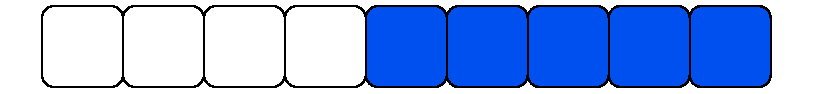
\includegraphics[width=\textwidth]{figuras/perfo_init.pdf}
        \caption{Comportamento do modificador \texttt{init}.}
        \label{fig:perfo_init}
    \end{minipage}
    \hfill

    \begin{minipage}[b]{0.80\textwidth}
        \centering
        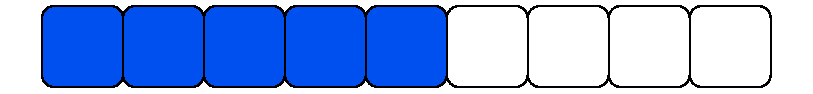
\includegraphics[width=\textwidth]{figuras/perfo_fini.pdf}
        \caption{Comportamento do modificador \texttt{fini}.}
        \label{fig:perfo_fini}
    \end{minipage}

    \begin{minipage}[b]{0.80\textwidth}
        \centering
        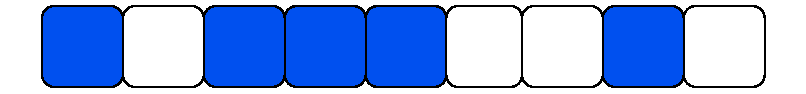
\includegraphics[width=\textwidth]{figuras/perfo_small.pdf}
        \caption{Comportamento do modificador \texttt{small}.}
        \label{fig:perfo_small}
    \end{minipage}

    \begin{minipage}[b]{0.80\textwidth}
        \centering
        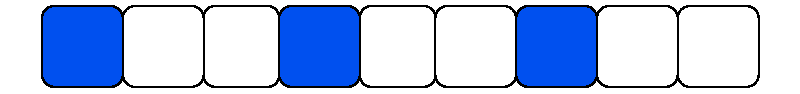
\includegraphics[width=\textwidth]{figuras/perfo_large.pdf}
        \caption{Comportamento do modificador \texttt{large}.}
        \label{fig:perfo_large}
    \end{minipage}

    \caption{Característica de cada modificador do \texttt{large}.}
    \label{fig:exemploMinipage}
\end{figure}

\section{Aproximação de ponto flutuante}\label{subsec:pragmaFastmath}

A cláusula \texttt{fastmath} habilita otimizações de ponto flutuante, seguindo a semântica do parâmetro de compilação \texttt{--fast-math} do compilador \texttt{Clang}~\cite{clangffast}. Quando aplicada, o compilador extrai a região de código anotada e adiciona metadados indicando que essa região permite otimizações agressivas de ponto flutuante.

A principal diferença entre os dois métodos está no fato de que a cláusula \texttt{fastmath} oferece controle mais granular, permitindo que as otimizações sejam aplicadas apenas na região especificada. Em contraste, o parâmetro global \texttt{--fast-math} força a aplicação dessas otimizações em todo o módulo de compilação. A \autoref{code:pragmaFastmath} apresenta a sintaxe da cláusula.

\begin{sourcecode}[htb]\caption{\label{code:pragmaFastmath}Sintaxe da cláusula \texttt{fastmath}}
    \begin{lstlisting}[frame=single, language=C++]
        #pragma omp approx fastmath
    \end{lstlisting}
    \fonte{}
\end{sourcecode}
Uma característica fundamental dessa cláusula está nas otimizações relacionadas à associatividade das operações de ponto flutuante. Isso permite que o compilador reordene operações de modo a melhorar o desempenho. Embora a reordenação seja válida para números reais, na aritmética de ponto flutuante ela pode produzir resultados numericamente distintos devido aos erros de arredondamento acumulados em cada operação. Esse comportamento é ilustrado na \autoref{fig:floatPoint}.

A \autoref{code:exFastmath} apresenta um exemplo prático do uso da cláusula. A função \textit{sqrt}, por exemplo, normalmente requer verificações adicionais para lidar com entradas inválidas, como valores negativos ou \textit{NaN} (\textit{Not a Number}). Ao aplicar \texttt{fastmath}, o compilador assume que essas entradas não ocorrerão, emitindo diretamente a instrução de hardware \textit{sqrt}, sem checagens extras, o que reduz a sobrecarga e melhora o desempenho.

\begin{sourcecode}[htb]\caption{\label{code:exFastmath}Sintaxe da clausula \texttt{fastmath}}
    \begin{lstlisting}[frame=single, language=C++]
        float sqrt_approx(float x)
        {
            #pragma omp approx fastmath
            {
                return sqrt(x);
            }
        }
    \end{lstlisting}
    \fonte{}
\end{sourcecode}

\section{Descarte de Tarefas}\label{subsec:pragmaTaskdrop}

O conceito de tarefas no \texttt{OpenMP} permite a execução assíncrona de regiões de código. Quando uma \textit{thread} encontra uma região anotada com a cláusula \texttt{task}, um objeto de tarefa é criado para ser executado posteriormente. Essa tarefa é então escalonada dinamicamente, podendo ser executada por qualquer outra \textit{thread}. Esse modelo de execução é particularmente útil em computações heterogêneas e irregulares, pois permite uma distribuição dinâmica da carga de trabalho entre as \textit{threads}~\cite{ayguade2007,openmpapi52}.

O construtor \texttt{taskloop} estende esse conceito para laços. Cada laço é particionado em pedaços, definidos pelo parâmetro \texttt{grainsize}, e uma tarefa é criada para cada pedaço. Essas tarefas podem então ser executadas de forma independente por diferentes \textit{threads}.

\begin{figure}[htb]
    \centering
    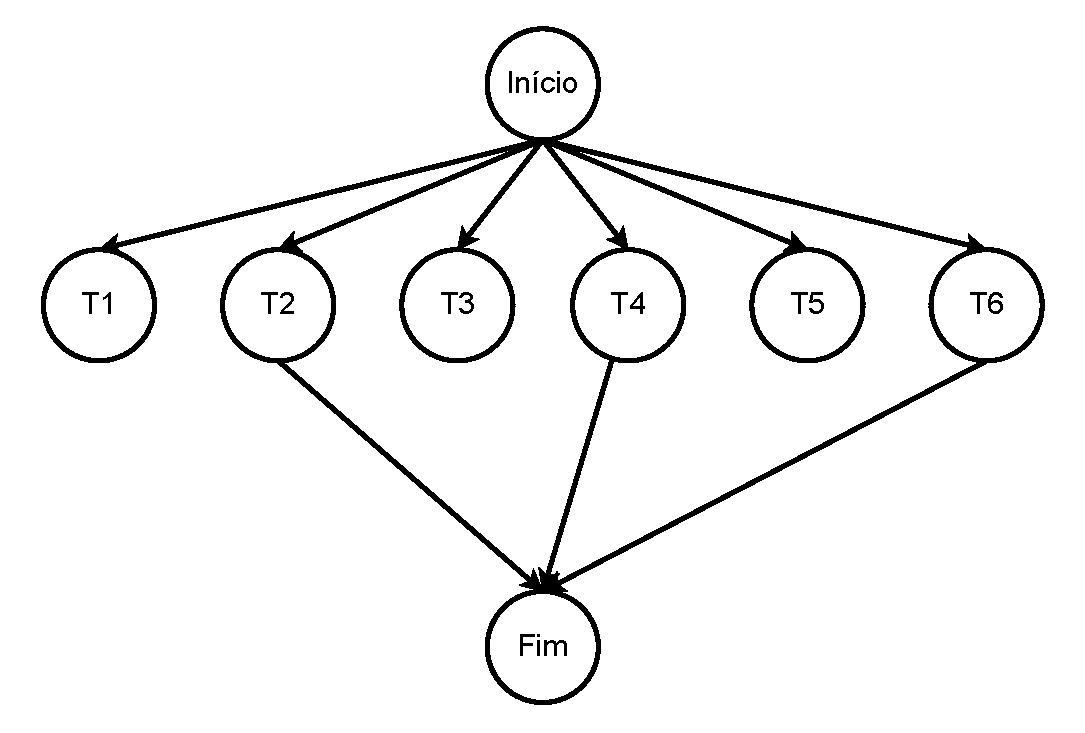
\includegraphics[width=\textwidth]{figuras/task.pdf}
    \caption{Modelo de execução da cláusula \texttt{drop}.}
    \label{fig:task_drop}
\end{figure}

Neste trabalho, propomos a cláusula \texttt{drop}, que pode ser usada em conjunto com \texttt{taskloop} para implementar uma estratégia de aproximação baseada no descarte de tarefas. De forma similar à técnica de perforação de laço, essa cláusula permite que o usuário especifique uma taxa de descarte, que define quantas tarefas serão eliminadas. A \autoref{eq:perfo} é utilizada para determinar quais tarefas devem ser descartadas.

A \autoref{fig:task_drop} ilustra esse processo, e o \autoref{code:pragmaDrop} apresenta a sintaxe da cláusula.

\begin{sourcecode}[htb]
    \caption{\label{code:pragmaDrop}Sintaxe da cláusula \texttt{drop}}
    \begin{lstlisting}[frame=single, language=C++]
        #pragma omp approx taskloop drop(drop-rate)
    \end{lstlisting}
    \fonte{}
\end{sourcecode}

O \autoref{code:exDrop} mostra um exemplo de uso da cláusula \texttt{drop} em conjunto com \texttt{taskloop} para aproximar o resultado de uma soma:

\begin{sourcecode}[htb]
    \caption{\label{code:exDrop}Exemplo de uso da cláusula \texttt{drop}}
    \begin{lstlisting}[frame=single, language=C++]
    #pragma omp parallel
    {
        #pragma omp single
        {
            #pragma omp approx taskloop drop(3) reduction(+ : sum)
            {
                for (int i = 0; i < N; i++) {
                    sum += values[i];
                }
            }
        }
    }
    \end{lstlisting}
    \fonte{}
\end{sourcecode}

\section{Memoização}\label{subsec:pragmaMemo}

A cláusula \texttt{memo} habilita otimizações de memoização, permitindo o reuso de resultados previamente calculados. Essa estratégia é particularmente útil para funções em que a relação entre entrada e saída se mantém estável ao longo do tempo, desde que a execução da mesma região de código produza resultados consistentes, independentemente das entradas específicas.

O \autoref{code:pragmaMemo} apresenta a sintaxe da cláusula \texttt{memo}. Essa cláusula deve ser utilizada em conjunto com a diretiva \texttt{shared} para garantir que, em tempo de execução, as variáveis indicadas possam ser acessadas. Opcionalmente, o modificador \texttt{threshold} pode ser especificado para definir um limite aceitável de erro entre os resultados que serão reutilizados.

\begin{sourcecode}[htb]
    \caption{\label{code:pragmaMemo}Sintaxe da cláusula \texttt{memo}}
    \begin{lstlisting}[frame=single, language=C++]
        #pragma omp approx memo shared([variables]) [threshold(error-limit)]
    \end{lstlisting}
    \fonte{}
\end{sourcecode}

\begin{figure}[htb]
    \centering
    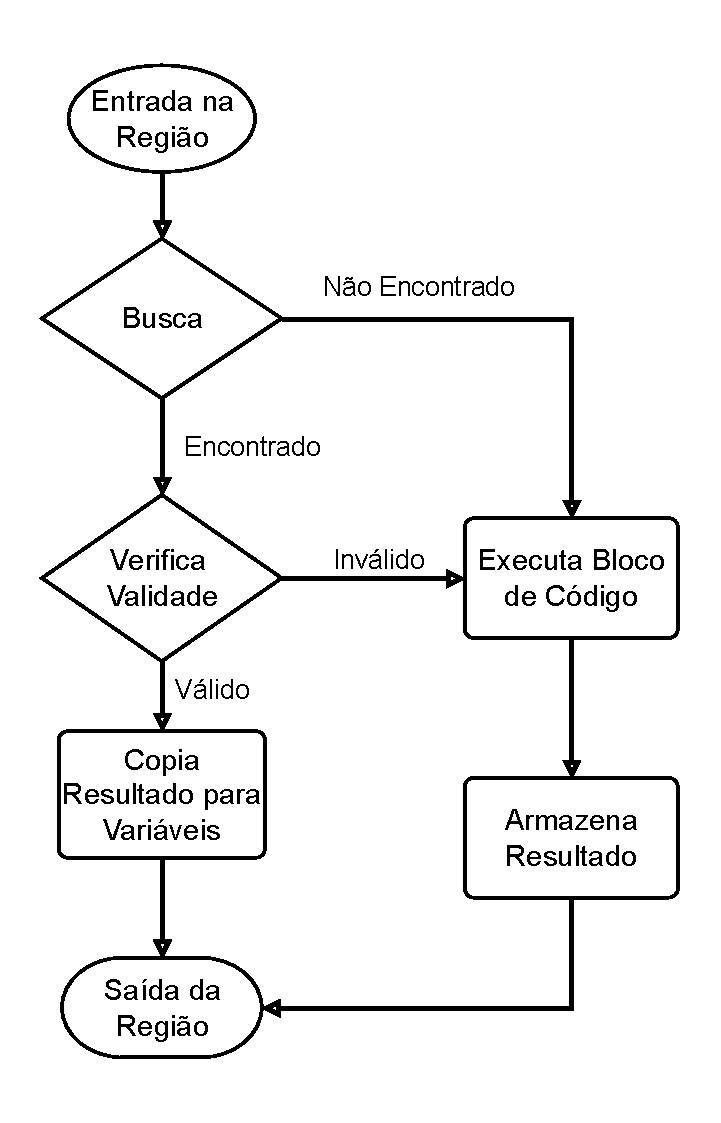
\includegraphics[scale=0.5]{figuras/memo.pdf}
    \caption{Modelo de execução da cláusula \texttt{memo}.}
    \label{fig:memo}
\end{figure}

Internamente, a técnica é implementada usando uma árvore AVL, cujos nós folha são estruturas \textit{hash map}. Em tempo de execução, as chamadas à função interceptam a região de código anotada e verificam se existe algum resultado previamente armazenado válido para aquela região. Se houver um resultado válido, ele é reutilizado; caso contrário, o bloco de código é executado normalmente e o resultado é armazenado para uso futuro. O fluxo de execução está ilustrado na \autoref{fig:memo}. É importante ressaltar que, nesta versão da implementação, a verificação de validade é feita exclusivamente com base na região de código, sem considerar diretamente os valores de entrada. Portanto, o reuso é determinado apenas pela execução da mesma região, independentemente das entradas fornecidas.

Quando o usuário especifica um limiar através do modificador \texttt{threshold}, a execução passa a incluir uma verificação que mede a diferença relativa entre os resultados da região. Se essa diferença estiver dentro do limite definido, o valor é armazenado e considerado válido para reuso. Caso nenhum limiar seja especificado, os valores previamente calculados são sempre reutilizados, sem verificação adicional. O \autoref{code:exMemo} apresenta um exemplo de uso da cláusula \texttt{memo} aplicado a um laço, usando um limiar de 10\%. Com a memoização habilitada, execuções repetidas dessa região de código podem ser substituídas por valores previamente calculados, respeitando o limite de erro definido.

\begin{sourcecode}[htb]
    \caption{\label{code:exMemo}Exemplo de uso da cláusula \texttt{memo}}
    \begin{lstlisting}[frame=single, language=C++]
        #pragma omp approx memo shared(sum) threshold(0.1)
        {
            for (int i = 0; i < N; i++) {
                sum += values[i];
            }
        }
    \end{lstlisting}
    \fonte{}
\end{sourcecode}


\chapter{Materiais e Métodos}\label{cap:metodologia}

Este capítulo apresenta a metodologia e os recursos utilizados no desenvolvimento deste trabalho. A \autoref{sec:config} descreve as configurações de \textit{hardware} das máquinas empregadas na execução dos experimentos. Em seguida, a \autoref{sec:benchmark} detalha as aplicações selecionadas para os testes, bem como as técnicas de otimização adotadas e o posicionamento das regiões paralelas. A \autoref{sec:desempenho} aborda os métodos utilizados para a coleta e análise dos dados de desempenho. Por fim, a \autoref{sec:resumo_exp} apresenta uma síntese de todos os experimentos realizados, organizada em formato tabular.

\section{Ambiente e Configuração Experimental}\label{sec:config}

Todos os experimentos deste trabalho foram realizados em um computador equipado com um processador Intel Core i7-4690, com frequência de 3.6 GHz, quatro núcleos físicos e suporte a oito \textit{threads}. A hierarquia de memória \textit{cache} apresenta 32 KB, 256 KB e 8 MB nos níveis L1, L2 e L3, respectivamente. O sistema possui 32 GB de memória RAM DDR3, distribuídos em quatro módulos de 8 GB configurados em \textit{dual-channel}, cada um operando a 1600 MT/s. O sistema operacional utilizado foi o Ubuntu 22.04 LTS. A \autoref{fig:compArchitecture} apresenta a hierarquia de memória e a disposição dos núcleos do processador utilizados nos testes.

\begin{figure}[htb]
	\caption{Especificação do computador utilizado em testes}
	\label{fig:compArchitecture}
	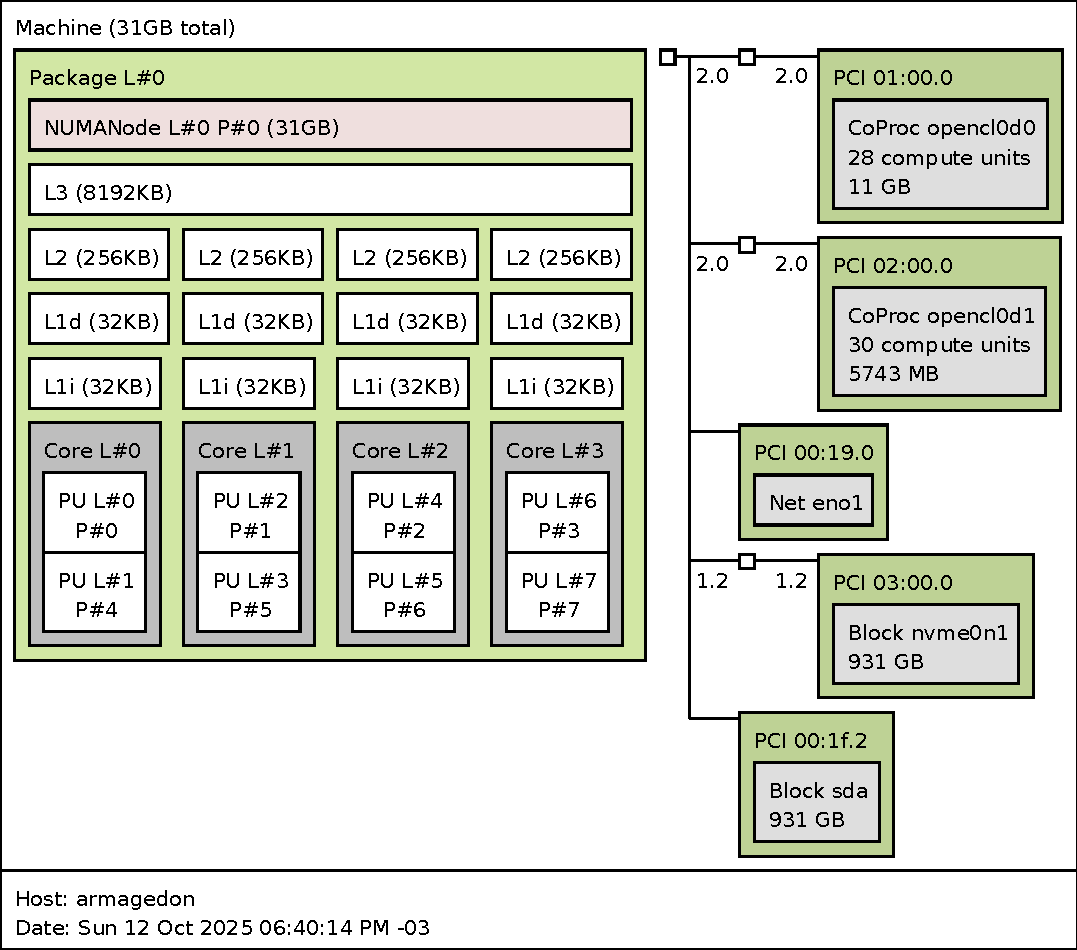
\includegraphics[scale=0.7]{figuras/architecture.pdf}
	\fonte{}
	\addcontentsline{loge}{figure}{\protect\numberline{\thefigure}Especificação do computador utilizado em testes.}
\end{figure}

Cada aplicação foi executada com diferentes quantidades de \textit{threads} (1, 2, 4 e 8), totalizando 10 execuções por configuração para reduzir variações no ambiente, todas compiladas com \textit{flag} de compilação \texttt{-O3} (nível de maior otimização do código gerado pelo compilador). Nos algoritmos que envolvem aleatoriedade, como \texttt{perfo} e \texttt{drop}, foi utilizada uma semente fixa para garantir a reprodutibilidade dos resultados. As técnicas \texttt{perfo}, \texttt{drop} e \texttt{memo} foram testadas com cinco níveis de taxa de exclusão: 0.1, 0.2, 0.3, 0.4 e 0.5.

\section{Conjunto de \textit{Benchmarks}}\label{sec:benchmark}

A seleção das aplicações que compõem o conjunto de benchmarks teve como principais critérios a tolerância a erros e a estrutura do algoritmo. Buscou-se contemplar uma gama ampla de domínios, incluindo \textit{machine learning}, álgebra linear, modelos estatísticos e multimídia. Outro objetivo foi preservar ao máximo o código original durante a inserção das regiões paralelizadas, evitando modificações significativas na implementação. Parte dessas aplicações foi obtida a partir do conjunto PolyBench~\cite{polybench}.

\subsection{2MM}\label{subsec:2mm}

2mm~\cite{polybench} é uma aplicação que realiza a multiplicação sequencial de duas matrizes, utilizando três matrizes distintas: $A$, $B$ e $C$. O processo de execução é ilustrado pelas equações \autoref{eq:dot_matrix_a} e \autoref{eq:dot_matrix_b}.

\begin{equation}
	\label{eq:dot_matrix_a}
	D = A \cdot B
\end{equation}

\begin{equation}
	\label{eq:dot_matrix_b}
	E = C \cdot D
\end{equation}

O algoritmo de multiplicação de matrizes empregado segue o padrão clássico~\cite{axler2015} descrito na \autoref{eq:multi_matrix}, que mostra a multiplicação de duas matrizes 2x2, representando o processo de somas e multiplicações sequenciais. A implementação utilizada pelo \textit{benchmark} é apresentada no \autoref{alg:mul_matrix}.

\begin{equation}
	\label{eq:multi_matrix}
	\begin{bmatrix}
		a_1 & a_2 \\
		a_3 & a_4
	\end{bmatrix}
	\cdot
	\begin{bmatrix}
		b_1 & b_2 \\
		b_3 & b_4
	\end{bmatrix}
	=
	\begin{bmatrix}
		a_1b_1 + a_2b_3 & a_1b_2 + a_2b_4 \\
		a_3b_1 + a_4b_3 & a_3b_2 + a_4b_4
	\end{bmatrix}
\end{equation}

\begin{algorithm}[htb]
	\caption{Multiplicação de matrizes}
	\label{alg:mul_matrix}
	\hrule
	\begin{algorithmic}[1]
		\REQUIRE Matrizes $A$ de tamanho $n \times m$, $B$ de tamanho $m \times p$, $C$ de tamanho $n \times p$
		\FOR{$i = 0$ até $n$, com passo $1$}
		\FOR{$j = 0$ até $p$, com passo $1$}
		\FOR{$k = 0$ até $m$, com passo $1$}
		\STATE $C[i][j] \gets C[i][j] + A[i][k] \cdot B[k][j]$
		\ENDFOR
		\ENDFOR
		\ENDFOR
	\end{algorithmic}
	\hrule
	\fonte{\citet{polybench}}
\end{algorithm}

Nesta aplicação, ambas as multiplicações são executadas em sequência, conforme as equações \autoref{eq:dot_matrix_a} e \autoref{eq:dot_matrix_b}. Para reduzir o \textit{overhead}, optou-se por utilizar uma única região paralela que abrange ambas multiplicações. Além da paralelização foi empregado a técnica de \textit{loop tiling}~\cite{bakos2016}. Essa técnica consiste em dividir o espaço de iteração em blocos menores, \textit{tiles}, de modo que cada bloco seja completamente processado antes de avançar para o próximo. Diferentemente da iteração convencional, que percorre toda uma dimensão por vez, no \textit{tiling} os acessos a memória são reorganizados para melhorar a localidade espacial e temporal.

O principal benefício dessa otimização está no uso mais eficiente da \textit{cache}. Idealmente, cada bloco deve ser dimensionado de forma que seus dados caibam inteiramente na \textit{cache}, permitindo que todo o bloco seja carregado e processado de uma só vez. Dessa forma, reduz-se o número de acessos à memória principal e evita-se o recarregamento de dados já utilizados, aumentando o desempenho da aplicação~\cite{bakos2016}. O \autoref{alg:tiling} apresenta o pseudocódigo de implementação dessa técnica na multiplicação de matrizes.

\begin{algorithm}[htb]
	\caption{Multiplicação de matrizes com \textit{loop tiling}}
	\label{alg:tiling}
	\hrule
	\begin{algorithmic}[1]
		\REQUIRE Matrizes $A$, $B$ e $C$ de tamanho $n \times n$
		\REQUIRE Tamanho do bloco $bs$
		\FOR{$ii = 0$ até $n$, com passo $bs$}
		\FOR{$kk = 0$ até $n$, com passo $bs$}
		\FOR{$i = ii$ até $\min(ii + bs, n)$}
		\FOR{$k = kk$ até $\min(kk + bs, n)$}
		\STATE $a\_val \gets A[i][k]$
		\FOR{$j = 0$ até $n$, com passo $1$}
		\STATE $C[i][j] \gets C[i][j] + a\_val \times B[k][j]$
		\ENDFOR
		\ENDFOR
		\ENDFOR
		\ENDFOR
		\ENDFOR
	\end{algorithmic}
	\hrule
	\fonte{}
\end{algorithm}

Outra técnica empregada, também utilizada nos demais benchmarks, foi a alocação contínua de memória. Em vez de alocar um bloco de memória separado para cada linha da matriz, foi alocado um único bloco contíguo. Esta técnica foi adotada visando á redução de chamadas de alocação e uma melhor da localidade espacial, contribuindo para um melhor desempenho.

\subsection{Correlação}\label{subsec:correlation}

A correlação é uma medida estatística que expressa o grau de associação entre duas variáveis~\cite{morettin2010}. Quando há correlação entre duas variáveis, isso indica que mudanças em uma delas tendem estar relacionadas a mudanças na outra.

A correlação pode ser positiva quando, ambas as variáveis aumentam ou diminuem juntas, ou negativa, quando uma variável aumenta enquanto a outra diminui. O valor da correlação varia de -1 a 1. Valores próximos de 1 indicam uma forte correlação positiva, enquanto valores próximos de -1, uma forte correlação negativa e valores próximos de 0 indicam uma fraca ou nenhuma correlação. A \autoref{fig:correlation}, ilustra esses três tipos de correlação, nos quais é possível observar visualmente o comportamento das variáveis em cada caso.

\begin{figure}[htb]
	\caption{Gráfico do cálculo de coeficiente de correlação de Pearson}
	\centering
	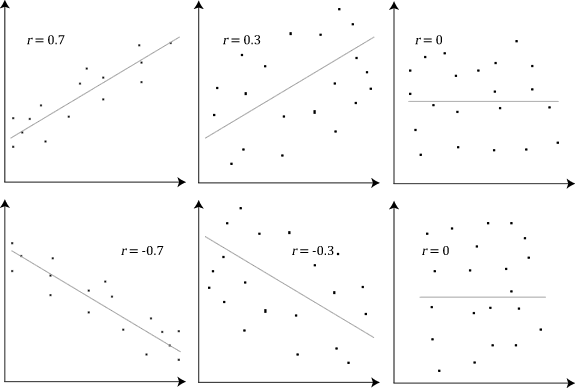
\includegraphics[scale=0.7]{figuras/correlation.png}
	\label{fig:correlation}
	\fonte{\citet{wikimediaCorrelation}}
	\addcontentsline{lof}{figure}{\protect\numberline{\thefigure}Gráfico do cálculo de coeficiente de correlação de Pearson}
\end{figure}

A fórmula comumente utilizada para calcular a correlação é chamada de \textit{Pearson Correlation Formula}, apresentada na \autoref{eq:correlation}~\cite{morettin2010}. Nessa equação, $x$ e $y$ representam os valores das variáveis, enquanto $m_x$ e $m_y$ correspondem as suas respectivas médias. A implementação utilizada pelo \textit{benchmark}~\cite{polybench} é apresentada em \autoref{alg:correlation_matrix} e \autoref{alg:correlation}, as quais são respectivamente o algoritmo para a construção da matriz de correlação e o cálculo do coeficiente em si.

\begin{equation}
	\label{eq:correlation}
	r = \frac{\sum(x - m_x)(y - m_y)}{\sqrt{\sum(x-m_x)^2 \sum(y - m_y)^2}}
\end{equation}

\begin{algorithm}[htb]
	\caption{Construção da matriz de correlação}
	\label{alg:correlation_matrix}
	\hrule
	\begin{algorithmic}[1]
		\REQUIRE Matrizes $C$ e $D$ de tamanho $n \times m$
		\FOR{$i = 0$ até $n$, com passo $1$}
		\FOR{$j = 0$ até $n$, com passo $1$}
		\IF{(j == i)}
		\STATE $r \gets 1.0$
		\ELSE
		\STATE $r \gets \texttt{correlation}(\texttt{linha}(D, i),\ \texttt{linha}(D, j),\ m)$
		\ENDIF
		\STATE $C[i][j] \gets r$
		\STATE $C[j][i] \gets r$
		\ENDFOR
		\ENDFOR
	\end{algorithmic}
	\hrule
	\fonte{}
\end{algorithm}

\begin{algorithm}[htb]
	\caption{Cálculo do coeficiente de correlação de Pearson}
	\label{alg:correlation}
	\hrule
	\begin{algorithmic}[1]
		\REQUIRE \textit{Array} $X$ e $Y$ de tamanho $m$
		\STATE $sumX \gets 0$
		\STATE $sumY \gets 0$
		\STATE $sumXY \gets 0$
		\STATE $sumX2 \gets 0$
		\STATE $sumY2 \gets 0$
		\FOR{$i = 0$ até $n$, em passos de $1$}
		\STATE $\texttt{sumX} \gets \texttt{sumX} + X[i]$
		\STATE $\texttt{sumY} \gets \texttt{sumY} + Y[i]$
		\STATE $\texttt{sumXY} \gets \texttt{sumXY} + X[i] * Y[i]$
		\STATE $\texttt{sumX2} \gets \texttt{sumX2} + X[i] * X[i]$
		\STATE $\texttt{sumY2} \gets \texttt{sumY2} + Y[i] * Y[i]$
		\ENDFOR
	\end{algorithmic}
	\hrule
	\fonte{}
\end{algorithm}

O cálculo da correlação entre as diferentes variáveis está apresentado na \autoref{tab:correlation}. Uma importante propriedade desse cálculo, está no fato de que ela é uma matriz simétrica, isto é, os valores localizados na parte inferior da matriz são iguais aos da parte superior em relação à diagonal principal. Essa diagonal principal contém valores iguais a $1.0$, correspondentes a autocorrelação perfeita de cada variável. Essa simetria permite otimizar o cálculo, reduzindo o número de iterações, uma vez que é suficiente computar os coeficientes para somente uma das metades da matriz.

\begin{table}[htb]
	\caption{Representação da correlação entre as diferentes variáveis}
	\centering
	\begin{tabular}{|c|c|c|c|c|}
		\hline
		           & \textbf{a} & \textbf{b} & \textbf{c} & \textbf{d} \\
		\hline
		\textbf{a} & 1.0        & ab         & ac         & ad         \\
		\hline
		\textbf{b} & ab         & 1.0        & bc         & bd         \\
		\hline
		\textbf{c} & ac         & bc         & 1.0        & cd         \\
		\hline
		\textbf{d} & ad         & bd         & cd         & 1.0        \\
		\hline
	\end{tabular}
	\fonte{}
	\label{tab:correlation}
\end{table}

No \autoref{alg:correlation_matrix} é possível observar que essa propriedade de simétrica foi explorada, e é também nessa região de código, mais especificamente em seu laço mais externo, que foi adicionado as anotações de paralelização, permitindo que o cálculo dos coeficientes fossem executados concorrententemente.

\subsection{Deriche}\label{subsec:deriche}

\begin{algorithm}[htb]
	\caption{Algoritmo Deriche de suavização}
	\label{alg:deriche1d}
	\hrule
	\begin{algorithmic}[1]
		\REQUIRE Imagem $I_{in}$ de tamanho $h \times w$
		\REQUIRE Coeficiente de suavização $\alpha$
		\STATE $I_{out1} \gets$ nova Matriz $h \times w$
		\STATE $I_{out2} \gets$ nova Matriz $h \times w$
		\STATE $I_{final} \gets$ nova Matriz $h \times w$

		\COMMENT{Cálculo dos coeficientes de suavização}
		\STATE $k \gets \frac{(1 - e^{-\alpha})^2}{1 + 2\alpha e^{-\alpha} - e^{-2\alpha}}$
		\STATE $a_1 \gets k$
		\STATE $a_2 \gets k \cdot e^{-\alpha} \cdot (\alpha - 1)$
		\STATE $a_3 \gets k \cdot e^{-\alpha} \cdot (\alpha + 1)$
		\STATE $a_4 \gets -k \cdot e^{-2\alpha}$
		\STATE $b_1 \gets 2 \cdot e^{-\alpha}$
		\STATE $b_2 \gets -e^{-2\alpha}$

		\COMMENT{Varredura horizontal (esquerda para direita)}
		\FOR{$i = 0$ até $h - 1$, com passo $1$}
		\STATE $y_{m1} \gets 0$, $y_{m2} \gets 0$
		\FOR{$j = 0$ até $w - 1$, com passo $1$}
		\STATE $I_{out1}[i, j] \gets a_1 \cdot I_{in}[i, j] + a_2 \cdot I_{in}[i, j-1] + b_1 \cdot y_{m1} + b_2 \cdot y_{m2}$
		\STATE $y_{m2} \gets y_{m1}$
		\STATE $y_{m1} \gets I_{out1}[i, j]$
		\ENDFOR
		\ENDFOR

		\COMMENT{Varredura horizontal (direita para esquerda)}
		\FOR{$i = 0$ até $h - 1$, com passo $1$}
		\STATE $y_{p1} \gets 0$, $y_{p2} \gets 0$
		\FOR{$j = w - 1$ até $0$, com passo $-1$}
		\STATE $I_{out2}[i, j] \gets a_3 \cdot I_{in}[i, j+1] + a_4 \cdot I_{in}[i, j+2] + b_1 \cdot y_{p1} + b_2 \cdot y_{p2}$
		\STATE $y_{p2} \gets y_{p1}$
		\STATE $y_{p1} \gets I_{out2}[i, j]$
		\ENDFOR
		\ENDFOR

		\COMMENT{Combinação final}
		\STATE $I_{final} \gets I_{out1} + I_{out2}$

		\RETURN $I_{final}$
	\end{algorithmic}
	\hrule
\end{algorithm}

Em processamento de imagens, o filtro de Deriche é um algoritmo de filtragem recursiva utilizado tanto para suavização de imagens quanto para detecção de bordas~\cite{deriche1987}. Este algoritmo foi desenvolvido como uma otimização do detector de bordas de Canny, buscando aproximar as propriedades de um filtro Gaussiano, por meio de um filtro \gls{iir}.

De forma intuitiva, o filtro de Deriche funciona de maneira diferente de um filtro baseado em uma janela fixa de pixels. Nesse algoritmo, os resultados intermediários de pixels anteriores são armazenados e são utilizados no cálculo dos pixels seguintes. O filtro percorre a imagem duas vezes, primeiramente na horizontal, da esquerda para a direita, e depois da direita para a esquerda, aplicando recursivamente os valores anteiores. Esse procecsso resulta em uma suavização eficiente, mantendo contornos suaves nas bordas da figura.

O nível dessa suavização é controlado pelo parâmetro $\alpha$, que ajusta a supressão de ruído e a precisão na localização da borda. Esse parâmetro define os coeficientes $a$ e $b$, que são utilizados tanto na \autoref{eq:deriche_esq} e \autoref{eq:deriche_dir}, que são aplicados respectivamente da esquerda para a direita e da direita para a esquerda.

\begin{equation}
	\label{eq:deriche_esq}
	y^1_{ij} = a_1x_{ij} + a_2x_{ij - 1} + b_1y^1_{ij - 1} + b_2y^1_{ij - 2}
\end{equation}

\begin{equation}
	\label{eq:deriche_dir}
	y^2_{ij} = a_3x_{ij + 1} + a_4x_{ij + 2} + b_1y^2_{ij + 1} + b_2y^2_{ij + 2}
\end{equation}

O filtro implementado segue o padrão do \textit{benchmarks}~\cite{polybench}, ou seja, apenas a suavização foi implementada, não há uma geração das bordas da imagem. O \autoref{alg:deriche}, apresenta a implementação desse algoritmo de suavização, na alteração desse \textit{benchmark} foi adicionado uma região paralela que englobava todos os laços do algoritmo.

\begin{figure}[htbp]
	\caption{Aplicação do filtro de Deriche.}
	\centering
	\subfloat[Imagem original]{
		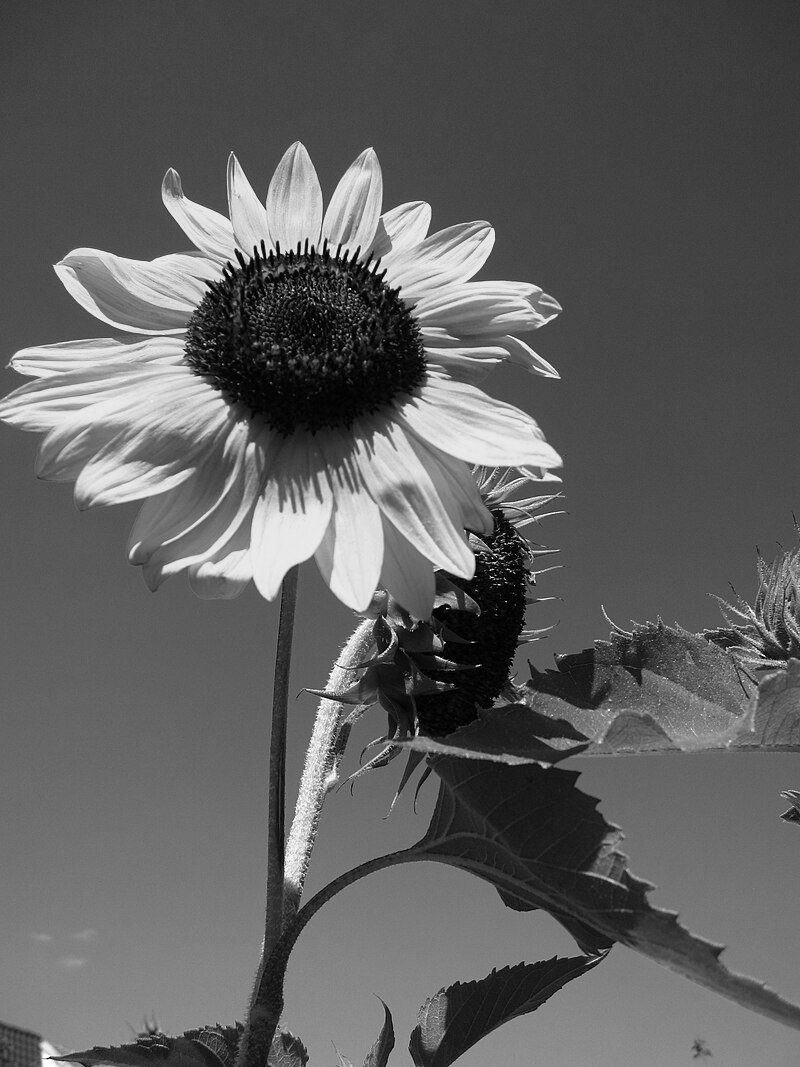
\includegraphics[width=0.45\textwidth]{sunflower_orig.jpg}
		\label{subfig:sunflower_orig}
	}
	\hfill
	\subfloat[Imagem com Deriche aplicado]{
		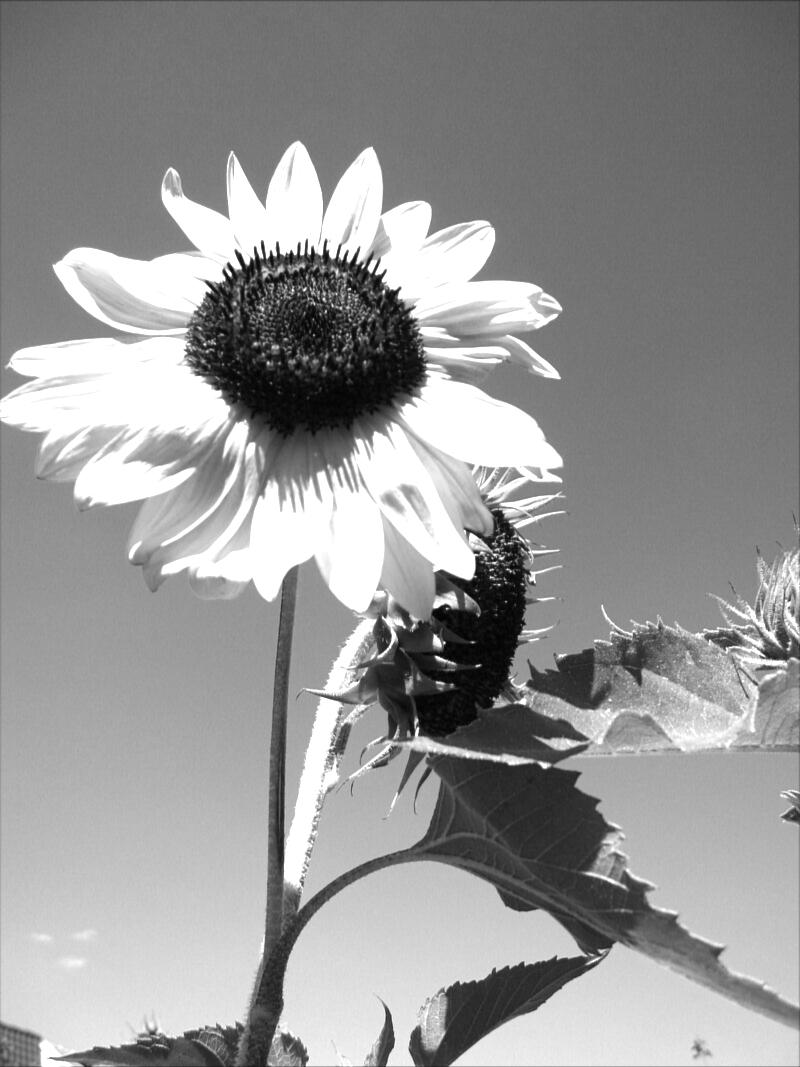
\includegraphics[width=0.45\textwidth]{sunflower_deri.jpg}
		\label{subfig:sunflower_deri}
	}
	\fonte{}
	\label{fig:deriche}
\end{figure}

A aplicação desse filtro com um $\alpha = 1.5$ em uma imagem pode ser observado na \autoref{fig:deriche}, aqui temos a \autoref{subfig:sunflower_orig} como sendo a imagem original em preto e branco e a \autoref{subfig:sunflower_deri} com o filtro aplicado. É possível perceber o como o filtro suaviza as bordas das imagens, tornando mais simples o processo de detecção de bordas.

\subsection{Jacobi 2D}\label{subsec:jacobi2d}

Em análise numérica, o método de Jacobi é um algoritmo iterativo utilizado para resolver sistemas de equações lineares do tipo $Ax = b$~\cite{szep2007}. Para que o método funcione adequadamente, o sistema deve atender a algumas condições específicas:

\begin{itemize}
	\item \textbf{Matriz quadrada:} A matriz dos coeficientes deve ser quadrada, ou seja, possuir o mesmo número de linhas e colunas;
	\item \textbf{Sistema linear:} O método aplica-se exclusivamente a sistemas lineares, ou seja, não deve haver termos como multiplicação entre variáveis ($xy$), potências superiores a 1 ($x^2$, $y^3$, etc.), nem funções não lineares, como seno, cosseno ou exponenciais ($e^x$);
	\item \textbf{Diagonal dominante:} Embora não seja uma exigência absoluta, a presença de dominância diagonal na matriz dos coeficientes é altamente recomendada, pois contribui para a garantia de convergência do método. Em sua ausência, o processo iterativo pode apresentar convergência lenta ou até mesmo não convergir.
\end{itemize}

Esse algoritmo foi selecionado como parte do conjunto de \textit{benchmarks}~\cite{polybench} adotados neste trabalho por sua natureza iterativa e previsível em termos de comportamento computacional. O processo inicia-se com a atribuição de valores iniciais arbitrários ao vetor $x$. Em seguida, realiza-se uma iteração para calcular uma nova estimativa da solução, com base exclusivamente nos valores da iteração anterior. Esses novos valores são utilizados como entrada para a próxima iteração. Esse procedimento é repetido até que a diferença entre iterações consecutivas seja inferior a um limiar de tolerância pré-definido, indicando a convergência para uma solução estável.

\begin{figure}[htb]
	\caption{Execução do algoritmo de estêncil}
	\centering
	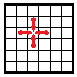
\includegraphics[scale=5]{figuras/jacobi2d.pdf}
	\label{fig:jacobi2d}
	\fonte{\citet{wikimediaJacobi2D}}
	\addcontentsline{lof}{figure}{\protect\numberline{\thefigure}Execução do algoritmo de estêncil}
\end{figure}

O Jacobi 2D é uma aplicação do método de Jacobi adaptado para problemas discretizados em duas dimensões. Sua implementação se baseia em um algoritmo de estêncil, no qual cada ponto de uma malha bidimensional é atualizado com base na média artimética dos seus quatro vizinhos imediatos (acima, abaixo, esquerda e a direita), como mostra a \autoref{fig:jacobi2d}. Após um número suficiente de iterações, a malha converge para uma configuração estável que representa uma aproximação da solução contínua do problema. O \autoref{alg:jacobi2d} apresenta a implementação utilizada pelo \textit{benchmark}.

\begin{algorithm}[htb]
	\caption{Método de Jacobi em duas dimensões}
	\label{alg:jacobi2d}
	\hrule
	\begin{algorithmic}[1]
		\REQUIRE Matriz $A$ e $B$ de tamanho $n \times n$
		\REQUIRE Quantidade de passos do algoritmo $p$
		\FOR{$t = 0$ até $p - 1$, com passo $1$}
		\FOR{$i = 1$ até $n - 1$, com passo $1$}
		\FOR{$j = 1$ até $n - 1$, com passo $1$}
		\STATE $B[i][j] \gets (A[i][j] + A[i][j + 1] + A[i][j - 1] + A[i - 1][j] + A[i + 1][j]) / 4$
		\ENDFOR
		\ENDFOR
		\FOR{$i = 1$ até $n - 1$, com passo $1$}
		\FOR{$j = 1$ até $n - 1$, com passo $1$}
		\STATE $A[i][j] \gets (B[i][j] + B[i][j + 1] + B[i][j - 1] + B[i - 1][j] + B[i+1][j]) / 4$
		\ENDFOR
		\ENDFOR
		\ENDFOR
	\end{algorithmic}
	\hrule
	\fonte{}
\end{algorithm}

O \autoref{alg:jacobi2d} apresenta dependência sequencial entre as etapas de atualização, o que dificulta a paralelização total. Para contornar isso, a paralelização foi aplicada no laço mais externo, permitindo que cada etapa de varredura seja executada em paralelo. Já os laços internos foram anotados com diretivas de sincronização, assegurando que os dados produzidos em uma etapa estejam disponíveis antes da próxima atualização.

\subsection{K-means}\label{subsec:kmeans}

O algoritmo K-means~\cite{macqueen1967} é uma técnica de agrupamento, que tem como objetivo particionar um conjunto de dados em $k$ grupos, de forma que os dados dentro de um mesmo grupo de modo que eles sejam semelhantes entre si.

\begin{algorithm}[htb!]
	\caption{Algoritmo K-means}
	\label{alg:kmeans}
	\hrule
	\begin{algorithmic}[1]
		\REQUIRE Matriz $features$ de dimensão $numPoints$ $\times$ $numFeatures$ \\
		\REQUIRE $numClusters$, número de $clusters$ que serão formados
		\REQUIRE $iterations$, quantidade de iterações realizada pelo algoritmo
		\REQUIRE $threshold$, limiar de parada do algoritmo

		\STATE Matriz $centroids$ de tamanho $numClusters \times numFeatures$, iniciado com $0$
		\STATE Matriz $newCentroids$ de tamanho $numClusters \times numFeatures$, iniciado com $0$
		\STATE \textit{Array} $membership$ de tamanho $numPoints$, iniciado com $-1$
		\STATE \textit{Array} $newCentroidsLen$ de tamanho $numClusters$, iniciado com $0$

		\FOR{$i = 0$ até $numClusters$, com passo $1$}
		\STATE $n \gets$ índice aleatório entre $0$ e $numPoints - 1$
		\FOR{$j = 0$ até $numFeatures$, com passo $1$}
		\STATE $\textit{centroids}[i][j] \gets \textit{features}[n][j]$
		\ENDFOR
		\ENDFOR

		\FOR{$iter = 0$ até $iterations$}
		\STATE $\textit{delta} \gets 0$

		\FOR{$j = 0$ até $numPoints$}
		\STATE $index \gets \texttt{find\_nearest\_point}(centroids, features[j], numFeatures)$

		\IF{$membership[j] \neq index$}
		\STATE $delta \gets delta + 1$
		\ENDIF

		\STATE $membership[j] \gets index$
		\STATE $newCentroidsLen[index] \gets newCentroidsLen[index] + 1$

		\FOR{$k = 0$ até $numFeatures$}
		\STATE $newCentroids[index][k] \gets newCentroids[index][k] + features[j][k]$
		\ENDFOR
		\ENDFOR

		\FOR{$j = 0$ até $numClusters$}
		\IF{$newCentroidsLen[j] > 0$}
		\FOR{$k = 0$ até $numFeatures$}
		\STATE $centroids[j][k] \gets newCentroids[j][k] / newCentroidsLen[j]$
		\ENDFOR
		\ENDIF
		\ENDFOR

		\STATE Zerar $newCentroids$
		\STATE Zerar $newCentroidsLen$

		\IF{$delta \leq threshold$}
		\STATE $break$
		\ENDIF
		\ENDFOR

		\RETURN  $centroids$
	\end{algorithmic}
	\hrule
	\fonte{}
\end{algorithm}

A ideia central do algoritmo consiste em definir inicialmente $k$ centróides, que são pontos de referência no espaço de amostragem. Em seguida, cada ponto de dado é associado ao centróide mais próximo, com base em uma medida de distância, usualmente a distância euclidiana. Após essa etapa de atribuição, o algoritmo calcula a média dos pontos atribuídos a cada grupo e atualiza a posição dos centróides com base nesses valores. A \autoref{fig:kmeans} ilustra o agrupamento dos dados ao longo das iterações do algoritmo K-means. Na figura, os triângulos representam os centróides, os pontos correspondem aos dados e as regiões coloridas indicam as áreas que delimitam os agrupamentos formados.

\begin{figure}[htb]
	\caption{Agrupamentos ao longo das iterações do algoritmo K-means}
	\centering
	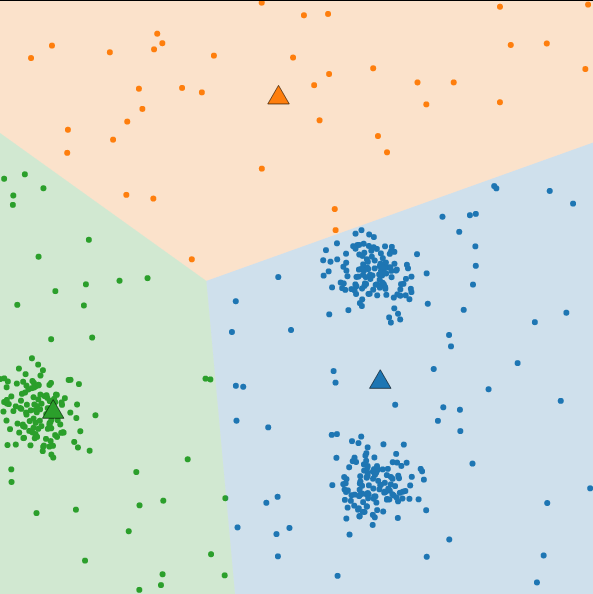
\includegraphics[scale=0.7]{figuras/kmeans.png}
	\label{fig:kmeans}
	\fonte{\citet{wikimediaKmeans}}
	\addcontentsline{lof}{figure}{\protect\numberline{\thefigure}Agrupamentos ao longo das iterações do algoritmo K-means}
\end{figure}

Esse processo é repetido iterativamente, os dados são reagrupados com base nos novos centróides e os centróides são novamente recalculados. O algoritmo continua até atingir um critério de parada, que pode ser um número fixo de iterações ou a estabilização dos centróides.

A \autoref{alg:kmeans}~\cite{rodinia} apresenta a implementação desse algoritmo, que reflete essa lógica de forma detalhada, incluindo a etapa de inicialização dos centróides, a atribuição de ponots, o recálculo dos centróides e a verificação do critério de parada

Durante a execução, o algoritmo também avalia a variância, uma medida que indica o quão disperso os pontos estão em relação ao seu centróide. Quanto menor essa variância, mais compactos são os grupos formados. Embora o objetivo não seja minimizar a variância até zero, uma variância excessivamente alta pode indicar que os dados não estão sendo agrupados de maneira eficiente.

Na implementação apresentada no \autoref{alg:kmeans}, a paralelização foi introduziada por meio de anotações dos laços internos, responsáveis pelas maiores cargas computacionais. Em particular, foram paralelizados os laços que percorrem os pontos de dados (\textit{numPoints}) e o laço que percorre os agrupamentos (\texttt{numclusters}).

\subsection{Mandelbrot}\label{subsec:mandelbrot}

\begin{figure}[htb]
	\caption{Representação do conjunto Mandelbrot}
	\centering
	\includegraphics[scale=0.15]{figuras/mandelbrot.png}
	\label{fig:mandelbrot}
	\fonte{}
	\addcontentsline{lof}{figure}{\protect\numberline{\thefigure}Representação do conjunto Mandelbrot}
\end{figure}

Mandelbrot é um conjunto de duas dimensções, definida no conjunto dos números complexos. Ele é construído a partir da iteração da função apresentada na \autoref{eq:mandelbrot}, onde $z$ e $c$ são números complexos, com $c$ constante para cada ponto avaliado e a condição inicial $z_0 = 0$~\cite{devaney1999}.

\begin{equation}
	\label{eq:mandelbrot}
	z_{n + 1} = z_n^{2} + c
\end{equation}

Nem todos os valores de $c$ pertencem ao conjunto de Mandelbrot. Um número complexo $c$ faz parte do conjunto se, ao aplicar a equação iterativamente, a sequência gerada não divergir, ou seja, os valores de $z_n$ permanencem no limite determinado mesmo após várias iterações. Na prática, considere-se que a sequência diverge quando $z_n > 2$, pois se isso continuará crescendo indefinidamente.

Para gerar a representação visual do conjunto Mandelbrot, mapeia-se cada pixel de uma imagem para um número complexo $c$. As regiões do plano onde $c$ pertence ao conjunto são então representadas visualmente.

Os valores de $c$ são escolhidos em um retângulo do plano complexo, com a parte real no intervalo $[-2, 1]$ e a parte imaginária em $[-1.5, 1.5]$. A conversão das coordenadas dos pixels para coordenadas no plano complexo é feita pelas equações \autoref{eq:mandelbrot_cx} e \autoref{eq:mandelbrot_cy}, onde $p_x$ e $p_y$ representam as coordenadas do pixel, e $x_{text{min}}$ e $x_{text{max}}$ definem o domínio da parte real, enquanto $y_{text{min}}$ e $y_{text{max}}$ definem o domínio da parte imaginária.

\begin{equation}
	\label{eq:mandelbrot_cx}
	c_x = x_{\text{min}} + \frac{p_x}{\text{largura da imagem}} \cdot (x_{\text{max}} - x_{\text{min}})
\end{equation}

\begin{equation}
	\label{eq:mandelbrot_cy}
	c_y = y_{\text{min}} + \frac{p_y}{\text{altura da imagem}} \cdot (y_{\text{max}} - y_{\text{min}})
\end{equation}

Inserimos os valores $c_x$ e $c_y$, nas iterações do Mandelbrot. Cada ponto da imagem é testado, e se a sequência $z_n$ não divergir após um número máximo de iterações, o pixel correspondente é colorido. A \autoref{fig:mandelbrot} apresenta uma visualização típica do conjunto de Mandelbrot. O \autoref{alg:mandelbrot}~\cite{debianBenchmarksGame} apresenta o cálculo do conjunto, e \autoref{alg:mandelbrot_image} contém o algoritmo utilizado para desenhar a imagem do conjunto.

\begin{algorithm}[htb]
	\caption{Cálculo do conjunto Mandelbrot}
	\label{alg:mandelbrot}
	\hrule
	\begin{algorithmic}[1]
		\REQUIRE Número complexo $c$
		\STATE $z \gets 0 + 0i$
		\FOR{$i = 0$ até $100$, com passo $1$}
		\STATE $z \gets z^2 + c$
		\IF{$|z| > 2.0$}
		\RETURN Falso
		\ENDIF
		\ENDFOR
		\RETURN Verdadeiro
	\end{algorithmic}
	\hrule
	\fonte{}
\end{algorithm}

\begin{algorithm}[htb]
	\caption{Geração da imagem do conjunto de Mandelbrot}
	\label{alg:mandelbrot_image}
	\hrule
	\begin{algorithmic}[1]
		\REQUIRE Tamanho da imagem base $n$
		\STATE $imageSize \gets (n / 8) \times 8$
		\STATE $pixels \gets$ vetor de tamanho $(imageSize \times imageSize) / 8$, inicializado com $0$
		\STATE $scaleX \gets (1.0 - (-2.0)) / imageSize$
		\STATE $scaleY \gets (1.5 - (-1.5)) / imageSize$

		\FOR{$pixel = 0$ até \texttt{tamanho}($pixels) - 1$}
		\STATE $byte \gets 0$
		\STATE $byteRow \gets imageSize / 8$
		\STATE $pixelColumn \gets pixel \bmod byteRow$
		\STATE $y \gets pixel / byteRow$

		\FOR{$bit = 0$ até $7$}
		\STATE $x \gets pixelColumn \times 8 + bit$
		\STATE $cx \gets -2.0 + x \times scaleX$
		\STATE $cy \gets -1.5 + y \times scaleY$
		\IF{$\texttt{mandelbrot}(cx,\ cy) =\ $Verdadeiro}
		\STATE $byte \gets byte\ |\ (1 \ll (7 - bit))$
		\ENDIF
		\ENDFOR

		\STATE $pixels[pixel] \gets byte$
		\ENDFOR
	\end{algorithmic}
	\hrule
	\fonte{}
\end{algorithm}

Na implementação apresentada, duas otimizações foram aplicadas, no \autoref{alg:mandelbrot_image}, com o objetivo de melhorar o desempenho do algoritmo. A primeira delas foi a adição de diretivas de paralelização, inseridas em seu laço mais externo, permitindo que diferentes regiões da imagem fossem processadas de forma concorrente.

A segunda otimização foi a aplicação da técnica conhecida como \textit{loop unrolling}, que consiste em transformar parte das iterações de um laço em instruções sequenciais explícitas. Essa técnica visa reduzir o overhead associado ao controle do laço, como verificações de condição e saltos, e pode beneficiar aspectos como \textit{branch prediction} e uso mais eficiente do \textit{pipeline} do processador.

\subsection{PI de Monte Carlo}\label{subsec:pi}

O método de Monte Carlo consiste em um conjunto de algoritmos estatísticos que utilizam amostragem aleatória para resolver problemas determinísticos ou estimar valores numérico~\cite{morettin2010}. Sua principal característica é a geração de entradas aleatórias dentro de um domínio previamente definido, seguido da aplicação de uma regra ou função para computar a saída, cujo resultados são então agregados para formar uma estimativa.

\begin{figure}[htb]
	\caption{Método de Monte Carlo}
	\centering
	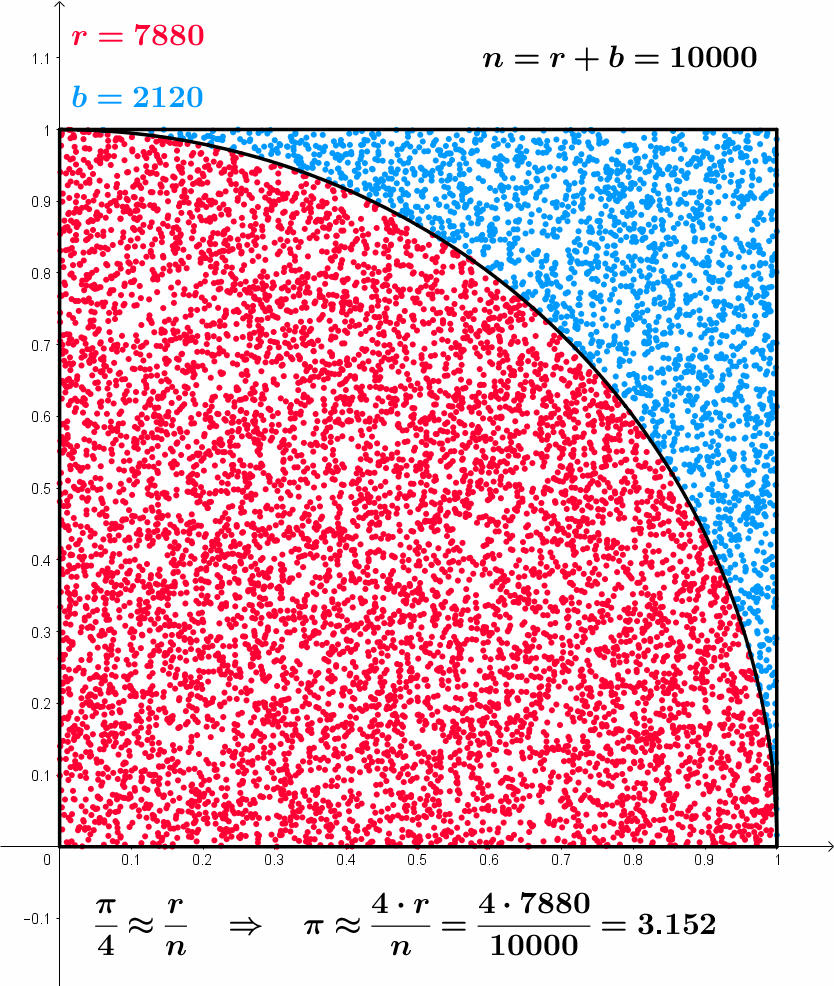
\includegraphics[scale=0.5]{figuras/pi.png}
	\label{fig:pi}
	\fonte{\citet{wikimediaPi}}
	\addcontentsline{lof}{figure}{\protect\numberline{\thefigure}Método de Monte Carlo}
\end{figure}

No caso específico da estimativa de $\pi$, o método pode ser aplicado de forma bastante intuitiva. Considere um cículo de raio $r = 1$, inscrito em um quadrado de lado $2$, conforme ilustrado na \autoref{fig:pi}. As áreas do círculo e do quadrado são dadas, respectivamente, pela \autoref{eq:area_circle} e \autoref{eq:area_square}. A razão entre essas duas áreas é apresentado na \autoref{eq:rational_area}. Por fim ao isolarmos o $\pi$, obtemos a \autoref{eq:rational_pi}.

\begin{equation}
	\label{eq:area_circle}
	A_{\text{círculo}} = \pi r^2 = \pi
\end{equation}

\begin{equation}
	\label{eq:area_square}
	A_{\text{quadrado}} = 2 \times 2 = 4
\end{equation}

\begin{equation}
	\label{eq:rational_area}
	\frac{A_{\text{círculo}}}{A_{\text{quadrado}}} = \frac{\pi}{4}
\end{equation}

\begin{equation}
	\label{eq:rational_pi}
	\pi = 4 \times \frac{A_{\text{círculo}}}{A_{\text{quadrado}}}
\end{equation}

A partir disso, é possível aplicar o método de Monte Carlo para estimar o valor de $\pi$. Como o círculo está inscrito no quadrado, o domínio de amostragem é o próprio quadrado. Gera-se então, um grande número de pontos aleatórios dentro do quadrado. Para cada ponto $(x, y)$, calcula-se sua distância até a origem. Se a distância for menor ou igual a 1, o ponto está dentro do círculo.

A estimativa de $\pi$ é obtida pela razão entre o número de pontos que caíram dentro do círculo e o número total de pontos gerados, multiplicada por 4, como mostra a \autoref{eq:pi_monte}, a \autoref{fig:pi} apresenta uma ilustração desse processo de amostragem e da aproximação de $\pi$. O \autoref{alg:pi} apresenta a implementação dessas equações utilizada no \textit{benchmark}.

\begin{equation}
	\label{eq:pi_monte}
	\pi \approx 4 \times \frac{\text{pontos dentro do círculo}}{\text{total de pontos}}
\end{equation}

\begin{algorithm}[htb]
	\caption{Cálculo de PI pelo método de Monte Carlo}
	\label{alg:pi}
	\hrule
	\begin{algorithmic}[1]
		\REQUIRE Quantidade de iterações $n$
		\STATE $hit \gets 0$
		\STATE $tid \gets \texttt{thread\_num}()$
		\STATE $seedState \gets \{tid, tid + 1\}$
		\FOR{$i = 0$ até $n$, com passo $1$}
		\STATE $x \gets \texttt{random}(seedState)$
		\STATE $y \gets \texttt{random}(seedState)$
		\IF{$(x \times x + y \times y) \leq 1$}
		\STATE $hit \gets hit + 1$
		\ENDIF
		\ENDFOR
		\RETURN $(4.0 \times hit) / n$
	\end{algorithmic}
	\hrule
	\fonte{}
\end{algorithm}

Na implementação apresentada no \autoref{alg:pi}, o laço principal foi paralelizado de forma que cada \textit{thread} execute uma fração do espaço total de iterações. Outra otimização introduzida nessa implementação, foi na geração de números pseudoaleatórios com o algoritmo \texttt{xorshift128+}, escolhido por sua alta velocidade e boa qualidade estatística.

\section{Análise de Desempenho}\label{sec:desempenho}

Para avaliar o impacto das otimizações propostas, foram conduzidos experimentos com as aplicações 2MM (sem a otimização de \textit{tiling}) e K-Means. Os testes foram executados variando o número de \textit{threads}, sendo testado com 1, 2, 4 e 8, com o objetivo de analisar os diferentes níveis de variação nos métodos de medição.

As medições foram realizadas utilizando a ferramenta \texttt{perf}, que permite coletar métricas de baixo nível do \textit{hardware} e do sistema operacional. Entre os principais eventos monitorados, destacam-se o número total de ciclos de CPU e o tempo total de execução das aplicações. Na \autoref{subfig:2mm_cycles_avg} e na \autoref{subfig:2mm_cycles_std} apresentam, respectivamente, a média de ciclos e o coeficiente de variação da aplicação 2MM. Já a \autoref{subfig:2mm_time_avg} e a \autoref{subfig:2mm_time_std} mostram a média do tempo de execução e o respectivo coeficiente de variação. O mesmo pode ser observado em relação ao K-Means, na \autoref{subfig:kmeans_cycles_avg} e na \autoref{subfig:kmeans_cycles_std}, que ilustram os resultados para os ciclos da aplicação, enquanto a \autoref{subfig:kmeans_time_avg} e a \autoref{subfig:kmeans_time_std} apresentam as medições referentes ao tempo de execução.

\begin{figure}[htbp]
	\caption{Medição de ciclos na aplicação 2MM.}
	\centering
	\subfloat[Média de ciclos]{
		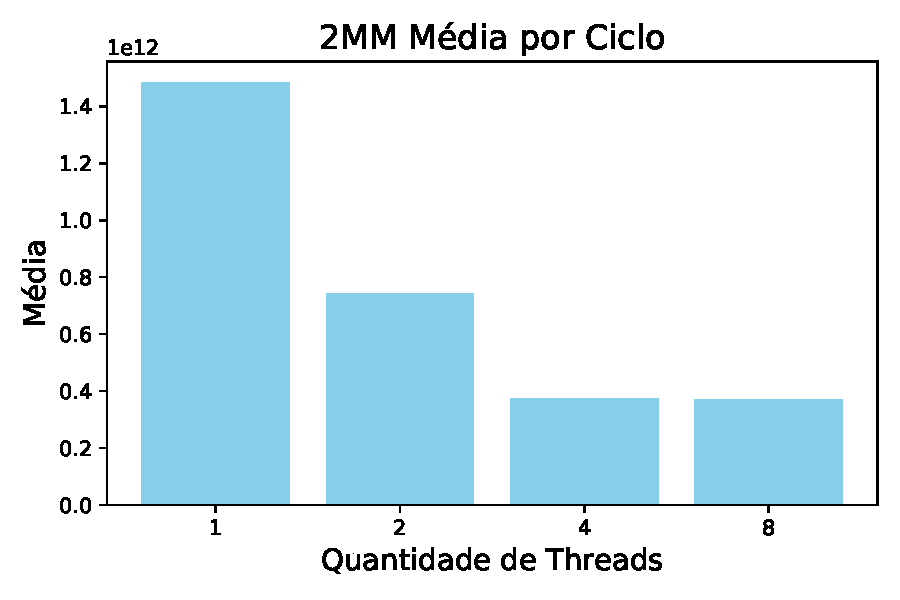
\includegraphics[width=0.45\textwidth]{2mm_cycles_avg.pdf}
		\label{subfig:2mm_cycles_avg}
	}
	\hfill
	\subfloat[Coeficiente de variação dos ciclos]{
		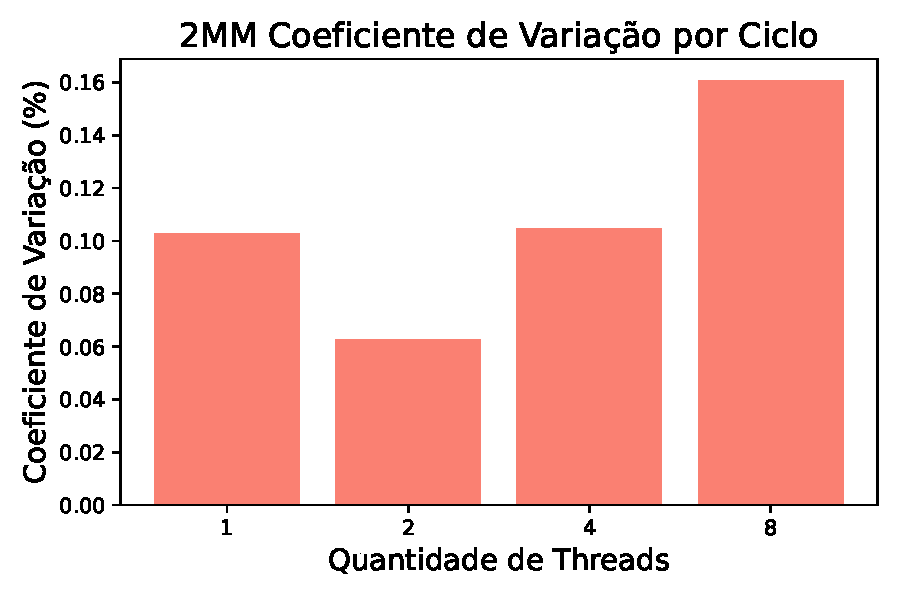
\includegraphics[width=0.45\textwidth]{2mm_cycles_std.pdf}
		\label{subfig:2mm_cycles_std}
	}
	\fonte{}
	\label{fig:2mm_cycles}
\end{figure}

\begin{figure}[htbp]
	\caption{Medição de ciclos na aplicação K-Means.}
	\centering
	\subfloat[Média de ciclos]{
		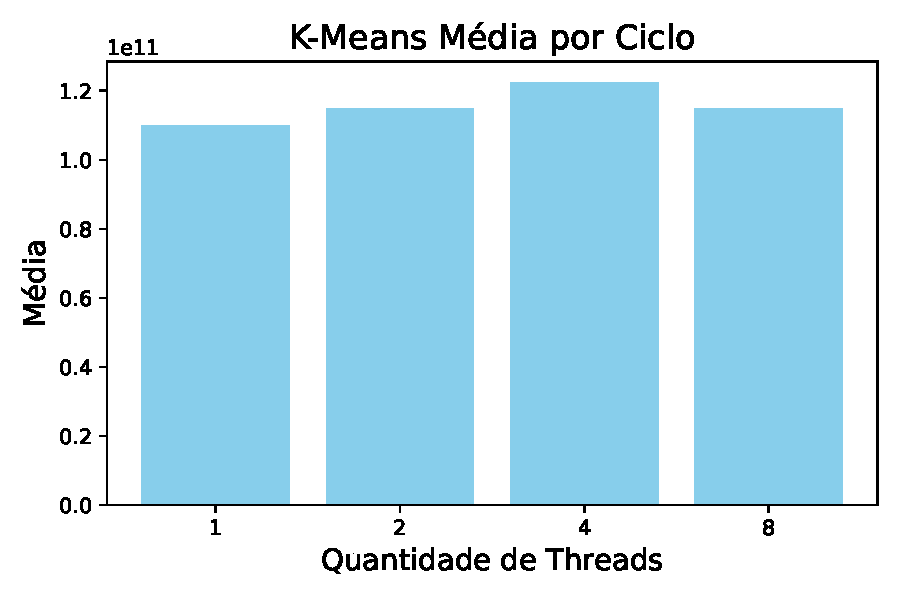
\includegraphics[width=0.45\textwidth]{kmeans_cycles_avg.pdf}
		\label{subfig:kmeans_cycles_avg}
	}
	\hfill
	\subfloat[Coeficiente de variação dos ciclos]{
		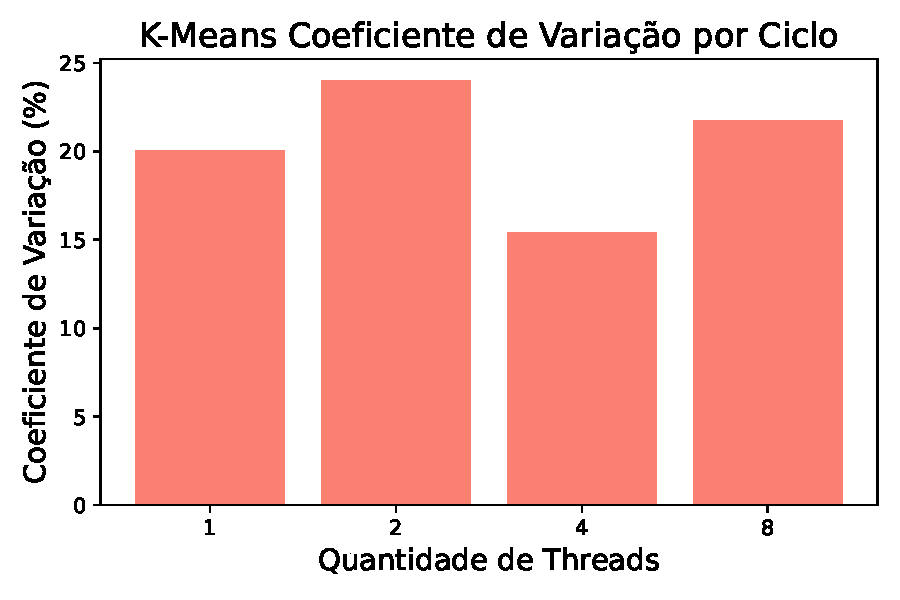
\includegraphics[width=0.45\textwidth]{kmeans_cycles_std.pdf}
		\label{subfig:kmeans_cycles_std}
	}
	\fonte{}
	\label{fig:kmeans_cycles}
\end{figure}

\begin{figure}[htbp]
	\caption{Medição de tempo na aplicação 2MM.}
	\centering
	\subfloat[Média de tempo]{
		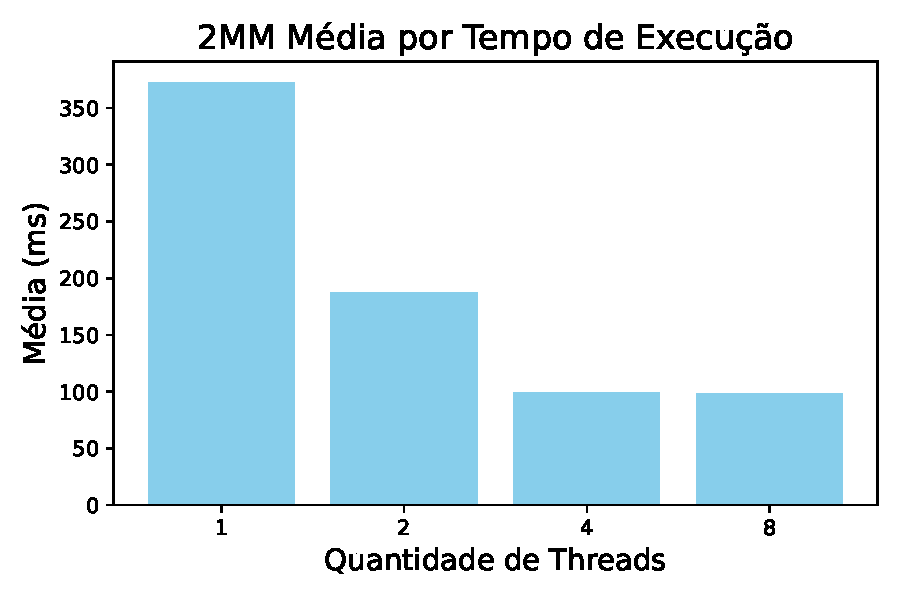
\includegraphics[width=0.45\textwidth]{2mm_time_avg.pdf}
		\label{subfig:2mm_time_avg}
	}
	\hfill
	\subfloat[Coeficiente de variação do tempo]{
		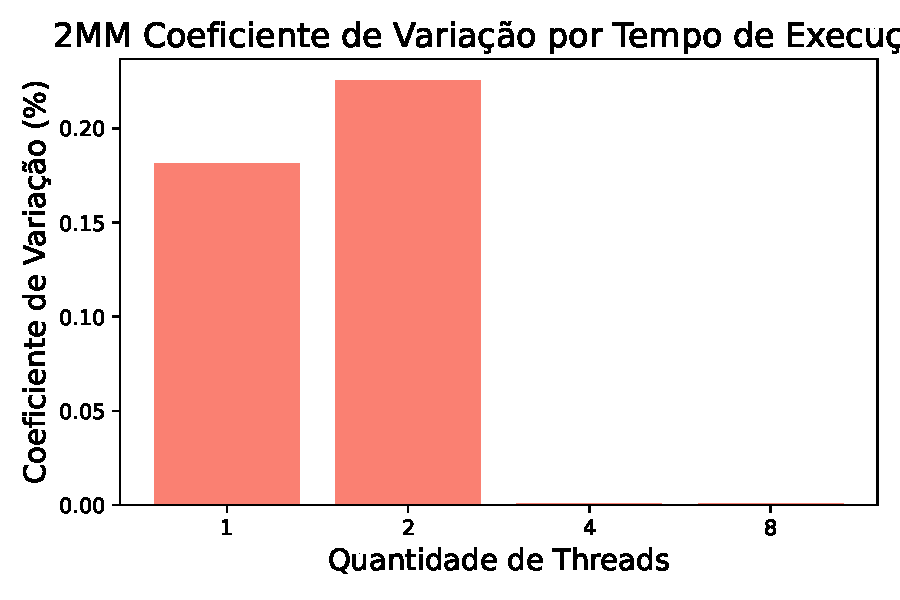
\includegraphics[width=0.45\textwidth]{2mm_time_std.pdf}
		\label{subfig:2mm_time_std}
	}
	\fonte{}
	\label{fig:2mm_time}
\end{figure}

\begin{figure}[htbp]
	\caption{Medição de tempo na aplicação K-Means.}
	\centering
	\subfloat[Média de tempo]{
		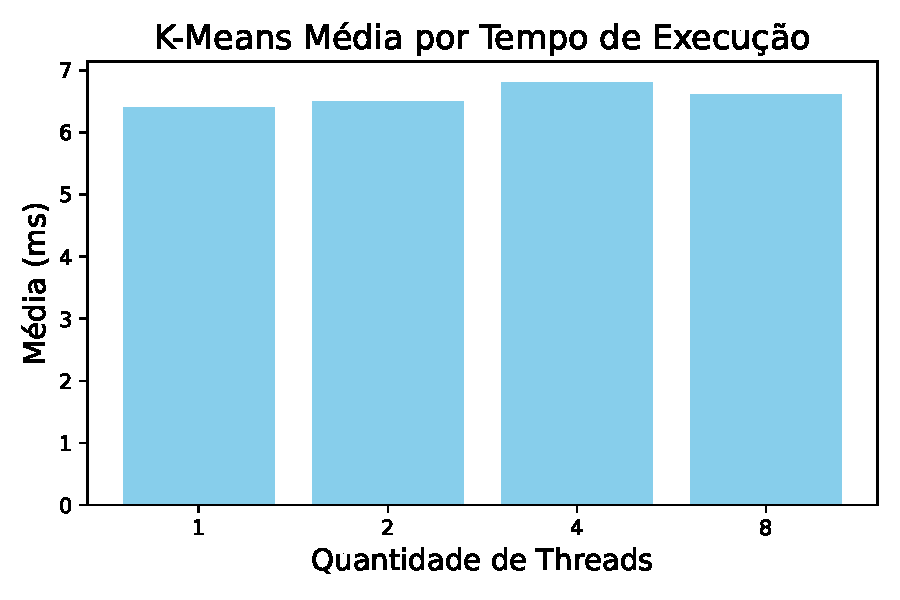
\includegraphics[width=0.45\textwidth]{kmeans_time_avg.pdf}
		\label{subfig:kmeans_time_avg}
	}
	\hfill
	\subfloat[Coeficiente de variação do tempo]{
		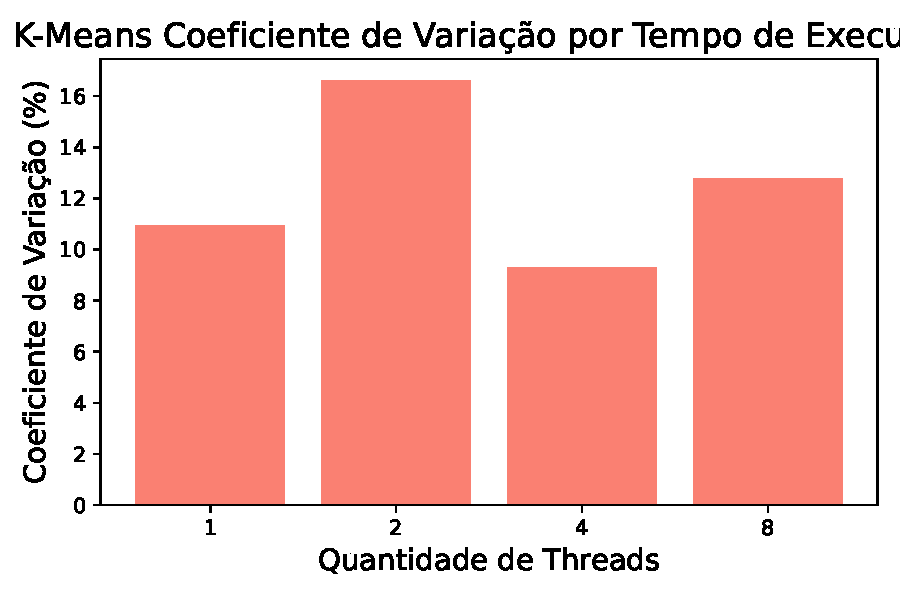
\includegraphics[width=0.45\textwidth]{kmeans_time_std.pdf}
		\label{subfig:kmeans_time_std}
	}
	\fonte{}
	\label{fig:kmeans_time}
\end{figure}

Com base nessa análise, optou-se por utilizar o tempo de execução como métrica principal para as medições de desempenho, uma vez que apresentou maior estabilidade entre as execuções e refletiu de forma mais consistente o comportamento das aplicações.

\section{Métricas de Qualidade}\label{sec:qualidade}

Para avaliar a perda de acurácia das aplicações, foram utilizadas três métricas distintas: o \gls{smape}, \gls{mcr} e o \gls{ssim}, definidos, respectivamente, em \autoref{eq:smape}, \autoref{eq:mcr} e \autoref{eq:ssim}.

\begin{equation}
	SMAPE(A, F) = \frac{100}{n} \sum^{n}_{t=1}\frac{|F_t - A_t|}{|A_t| + |F_t|}
	\label{eq:smape}
\end{equation}

\begin{equation}
	MCR(A, F) = \frac{1}{n} \sum^{n}_{t=1} \iota (A_t \neq F_t)
	\label{eq:mcr}
\end{equation}

Em que as variáveis são definidas como:
\begin{itemize}
	\item $n$: número de elementos no \textit{array} de dados;
	\item $A_t$: $t$-ésimo elemento obtido pela execução acurada;
	\item $F_t$: $t$-ésimo elemento obtido pela execução aproximada;
	\item $\iota$: função indicadora que retorna 1 quando a condição é verdadeira e 0 caso contrário.
\end{itemize}

\begin{equation}
	SSIM(x, y) = \frac{(2 \mu_x \mu_y + c_1) \cdot (2 \sigma_{xy} + c_2)}{(\mu_x^2 + \mu_y^2 + c_1) \cdot (\sigma_x^2 + \sigma_y^2 + c_2)}
	\label{eq:ssim}
\end{equation}

Em que as variáveis são definidas como:
\begin{itemize}
	\item $\mu_x$: média dos pixels da imagem $x$;
	\item $\mu_y$: média dos pixels da imagem $y$;
	\item $\sigma_x$: variância dos pixels da imagem $x$;
	\item $\sigma_y$: variância dos pixels da imagem $y$;
	\item $\sigma_y$: variância dos pixels da imagem $y$;
	\item $c_1$ e $c_2$: constante pequena para evitar divisão por $0$;
\end{itemize}

\section{Resumo dos \textit{Benchmarks}}\label{sec:resumo_exp}

\begin{table}[H]
	\centering
	\caption{Resumo das aplicações utilizadas nos experimentos}
	\begin{tabular}{|l|p{3.5cm}|l|l|}
		\hline
		\textbf{Aplicação} & \textbf{Fonte}                                     & \textbf{Domínio}            & \textbf{Métrica de Qualidade} \\
		\hline
		2MM                & PolyBench~\cite{polybench}                         & Álgebra Linear              & \gls{smape}                   \\
		\hline
		Correlação         & PolyBench~\cite{polybench}                         & Probabilidade e Estatística & \gls{smape}                   \\
		\hline
		Deriche            & PolyBench~\cite{polybench}                         & Processamento de Imagem     & \gls{ssim}                    \\
		\hline
		Jacobi 2D          & PolyBench~\cite{polybench}                         & Solução Numérica            & \gls{smape}                   \\
		\hline
		K-Means            & Rodinia~\cite{rodinia}                             & Aprendizado de Máquina      & \gls{mcr}                     \\
		\hline
		Mandelbrot         & Debian Benchmarks Game~\cite{debianBenchmarksGame} & Visualização Computacional  & \gls{smape}                   \\
		\hline
		PI de Monte Carlo  & Debian Benchmarks Game~\cite{debianBenchmarksGame} & Probabilidade e Estatística & \gls{smape}                   \\
		\hline
	\end{tabular}
	\fonte{}
	\label{tab:benchmarks}
\end{table}

Os \textit{benchmarks} definidos neste trabalho foram sumarizados na \autoref{tab:benchmarks}. Cada conjunto de testes teve como objetivo avaliar o desempenho e a acurácia das técnicas de aproximação implementadas.

\section{Cronograma}\label{sec:cronograma}

\begin{table}[htb]
	\centering
	\caption{Cronograma de execução das atividades}
	\begin{tabular}{|c|c|c|c|c|c|c|c|c|}
		\hline
		\textbf{Atividades} & \textbf{Ago} & \textbf{Set} & \textbf{Out} & \textbf{Nov} & \textbf{Dez} & \textbf{Jan} & \textbf{Fev} & \textbf{Mar} \\
		\hline
		1                   & X            & X            &              &              &              &              &              &              \\ \hline
		2                   &              & X            & X            &              &              &              &              &              \\ \hline
		3                   &              & X            & X            &              &              &              &              &              \\ \hline
		4                   &              &              & X            & X            &              &              &              &              \\ \hline
		5                   &              &              & X            & X            &              &              &              &              \\ \hline
		6                   &              &              & X            & X            &              &              &              &              \\ \hline
		7                   &              &              &              &              & X            & X            & X            &              \\ \hline
		8                   &              &              &              &              &              & X            & X            &              \\ \hline
		9                   &              &              &              &              &              &              & X            & X            \\ \hline
		10                  & X            & X            & X            & X            & X            & X            & X            & X            \\ \hline
	\end{tabular}
	\fonte{}
	\label{tab:cronograma}
\end{table}

A realização deste trabalho é organizada em partes, as quais são descritas a seguir:

\begin{enumerate}
	\item Realizar uma revisão da literatura relacionada à \gls{ca}, técnicas de aproximação e \gls{cp}.
	\item Revisar a infraestrutura do \texttt{OpenMP}.
	\item Investigar a infraestrutura do LLVM.
	\item Revisar aplicações de \textit{benchmark} que podem ser aplicadas em sistemas aproximados.
	\item Adaptar um \textit{benchmark suite} para que ele se encaixe nas otimizações paralelas e aproximadas.
	\item Testar e documentar as execuções dessas aplicações.
	\item Implementar técnicas de aproximação paralela na infraestrutura do \texttt{OpenMP} integrada ao LLVM.
	\item Testar e documentar as execuções do \textit{benchmark} em conjunto com as novas técnicas apresentadas.
	\item Investigar e avaliar o desempenho e a acurácia de cada uma das aplicações.
	\item Documentar todos os procedimentos e resultados.
\end{enumerate}

A \autoref{tab:cronograma} detalha o planejamento temporal para a execução de cada uma das atividades descritas.



%% Formatação de páginas de elementos pós-textuais
\postextual%% Não comente esta linha

%% Arquivos de referências
\arquivosdereferencias{%% Arquivos bibtex sem a extensão .bib e separados por vírgula - Não comente esta linha
  %./PosTexto/exemplos-referencias,%% Arquivo de referências - Comente para remover este item
  main%% Arquivo de referências - Comente para remover este item
}%% Não comente esta linha

%% Glossário
%\incluirglossario %% Comente para remover este item

%% Arquivos de apêndices
\begin{arquivosdeapendices}%% Os arquivos de apêndices devem se incluídos neste ambiente - Não comente esta linha
  %   %\partapendices%% Página de início dos apêndices - adiciona uma página com o título Apêndices
  %   %% Capítulo de exemplo
  %%%% APÊNDICE A
%%
%% Texto ou documento elaborado pelo autor, a fim de complementar sua argumentação, sem prejuízo da unidade nuclear do trabalho.

%% Título e rótulo de apêndice (rótulos não devem conter caracteres especiais, acentuados ou cedilha)
\chapter{Questionário de pesquisa}\label{cap:apendicea}

Quando houver necessidade pode-se apresentar como apêndice documento(s) auxiliar(es) e/ou complementar(es) como: legislação, estatutos, gráficos, tabelas, etc. Os apêndices são enumerados com letras maiúsculas: \autoref{cap:apendicea}, \autoref{cap:apendiceb}, etc.

No \latex\ apêndices são editados como capítulos. O comando \verb|\appendix| faz com que todos os capítulos seguintes sejam considerados apêndices.

Apêndices complementam o texto principal da tese com informações para leitores com especial interesse no tema, devendo ser considerados leitura opcional, ou seja, o entendimento do texto principal da tese não deve exigir a leitura atenta dos apêndices.

Apêndices usualmente contemplam provas de teoremas, deduções de fórmulas matemáticas, diagramas esquemáticos, gráficos e trechos de código. Quanto a este último, código extenso não deve fazer parte da tese, mesmo como apêndice. O ideal é disponibilizar o código na Internet para os interessados em examiná-lo ou utilizá-lo.

%% Título e rótulo de seção (rótulos não devem conter caracteres especiais, acentuados ou cedilha)
%\section{Título da Seção Secundária do Apêndice B}\label{sec:secaoapendicea}

%Exemplo de seção secundária em apêndice (\autoref{sec:secaoapendicea} do \autoref{cap:apendicea}).

%% Título e rótulo de seção (rótulos não devem conter caracteres especiais, acentuados ou cedilha)
%\subsection{Título da Seção Terciária do Apêndice B}\label{subsec:subsecaoapendicea}

%Exemplo de seção terciária em apêndice (\autoref{subsec:subsecaoapendicea} do \autoref{cap:apendicea}).

%% Título e rótulo de seção (rótulos não devem conter caracteres especiais, acentuados ou cedilha)
%\subsubsection{Título da seção quaternária do Apêndice B}\label{subsubsec:subsubsecaoapendicea}

%Exemplo de seção quaternária em apêndice (\autoref{subsubsec:subsubsecaoapendicea} do \autoref{cap:apendicea}).

%% Título e rótulo de seção (rótulos não devem conter caracteres especiais, acentuados ou cedilha)
%\paragraph{Título da seção quinária do Apêndice B}\label{para:paragraphapendicea}

%Exemplo de seção quinária em apêndice (\autoref{para:paragraphapendicea} do \autoref{cap:apendicea}).
%% Apêndice - Comente para remover este item
  %%%% APÊNDICE B
%%
%% Texto ou documento elaborado pelo autor, a fim de complementar sua argumentação, sem prejuízo da unidade nuclear do trabalho.

%% Título e rótulo de apêndice (rótulos não devem conter caracteres especiais, acentuados ou cedilha)
\chapter{Roteiro da entrevista}\label{cap:apendiceb}

\begin{table}[htb]%% Ambiente table
\caption{Orçamento dos materiais n.\textsuperscript{o} 1.}%% Legenda
\label{tab:tab3}%% Rótulo
\begin{tabularx}{\textwidth}{@{\extracolsep{\fill}}lrrr}%% Ambiente tabularx
\toprule
Material              & \multicolumn{1}{c}{Valor (R\$)} & \multicolumn{1}{c}{Quantidade}  & \multicolumn{1}{c}{Total (R\$)} \\ \midrule
Bomba centrífuga      & 2500,00                         & 01                              & 2500,00                         \\
Compressor rotativo   & 3000,00                         & 01                              & 3000,00                         \\
Manômetro diferencial & 450,00                          & 02                              & 900,00                          \\
Termopar              & 370,00                          & 02                              & 740,00                          \\
Válvula de esfera     & 43,00                           & 02                              & 86,00                           \\
Tubulação de PVC      & 10,00                           & 05                              & 50,00                           \\
Conexão de PVC        & 5,00                            & 10                              & 50,00                           \\ \midrule
                      &                                 & \multicolumn{1}{r}{Total (R\$)} & 7326,00                         \\ \bottomrule
\end{tabularx}
\fonte{}%% Fonte
\end{table}

\begin{table}[htb]%% Ambiente table
\caption{Orçamento dos materiais n.\textsuperscript{o} 2.}%% Legenda
\label{tab:tab4}%% Rótulo
\begin{tabularx}{\textwidth}{@{\extracolsep{\fill}}lrrr}%% Ambiente tabularx
\toprule
Material              & \multicolumn{1}{c}{Valor (R\$)} & \multicolumn{1}{c}{Quantidade}  & \multicolumn{1}{c}{Total (R\$)} \\ \midrule
Bomba centrífuga      & 2700,00                         & 01                              & 2700,00                         \\
Compressor rotativo   & 2950,00                         & 01                              & 2950,00                         \\
Manômetro diferencial & 515,00                          & 02                              & 1030,00                         \\
Termopar              & 350,00                          & 02                              & 700,00                          \\
Válvula de esfera     & 40,00                           & 02                              & 80,00                           \\
Tubulação de PVC      & 8,00                            & 05                              & 40,00                           \\
Conexão de PVC        & 6,00                            & 10                              & 60,00                           \\ \midrule
                      &                                 & \multicolumn{1}{r}{Total (R\$)} & 7560,00                         \\ \bottomrule
\end{tabularx}
\fonte{}%% Fonte
\end{table}

\begin{table}[htb]%% Ambiente table
\caption{Orçamento dos materiais n.\textsuperscript{o} 3.}%% Legenda
\label{tab:tab5}%% Rótulo
\begin{tabularx}{\textwidth}{@{\extracolsep{\fill}}lrrr}%% Ambiente tabularx
\toprule
Material              & \multicolumn{1}{c}{Valor (R\$)} & \multicolumn{1}{c}{Quantidade}  & \multicolumn{1}{c}{Total (R\$)} \\ \midrule
Bomba centrífuga      & 2600,00                         & 01                              & 2600,00                         \\
Compressor rotativo   & 3100,00                         & 01                              & 3100,00                         \\
Manômetro diferencial & 500,00                          & 02                              & 1000,00                         \\
Termopar              & 400,00                          & 02                              & 800,00                          \\
Válvula de esfera     & 45,00                           & 02                              & 90,00                           \\
Tubulação de PVC      & 12,00                           & 05                              & 60,00                           \\
Conexão de PVC        & 5,00                            & 10                              & 50,00                           \\ \midrule
                      &                                 & \multicolumn{1}{r}{Total (R\$)} & 7700,00                         \\ \bottomrule
\end{tabularx}
\fonte{}%% Fonte
\end{table}
%% Apêndice - Comente para remover este item
\end{arquivosdeapendices}%% Não comente esta linha


% \begin{apendicesenv}%% Ambiente apendicesenv

% \lipsum[55-56]

% \end{apendicesenv}

%% Arquivos de anexos
\begin{arquivosdeanexos}%% Os arquivos de anexos devem se incluídos neste ambiente - Não comente esta linha
  %\partanexos%% Página de início dos anexos - adiciona uma página com o título Anexos

  %%%% ANEXO A
%%
%% Texto ou documento não elaborado pelo autor, que serve de fundamentação, comprovação e ilustração.

%% Título e rótulo de anexo (rótulos não devem conter caracteres especiais, acentuados ou cedilha)
\anexos
\chapter{Lei N\texorpdfstring{.\textsuperscript{o}}{o.} 9.610, de 19 de Fevereiro de 1998}\label{cap:anexoa}

\centerline{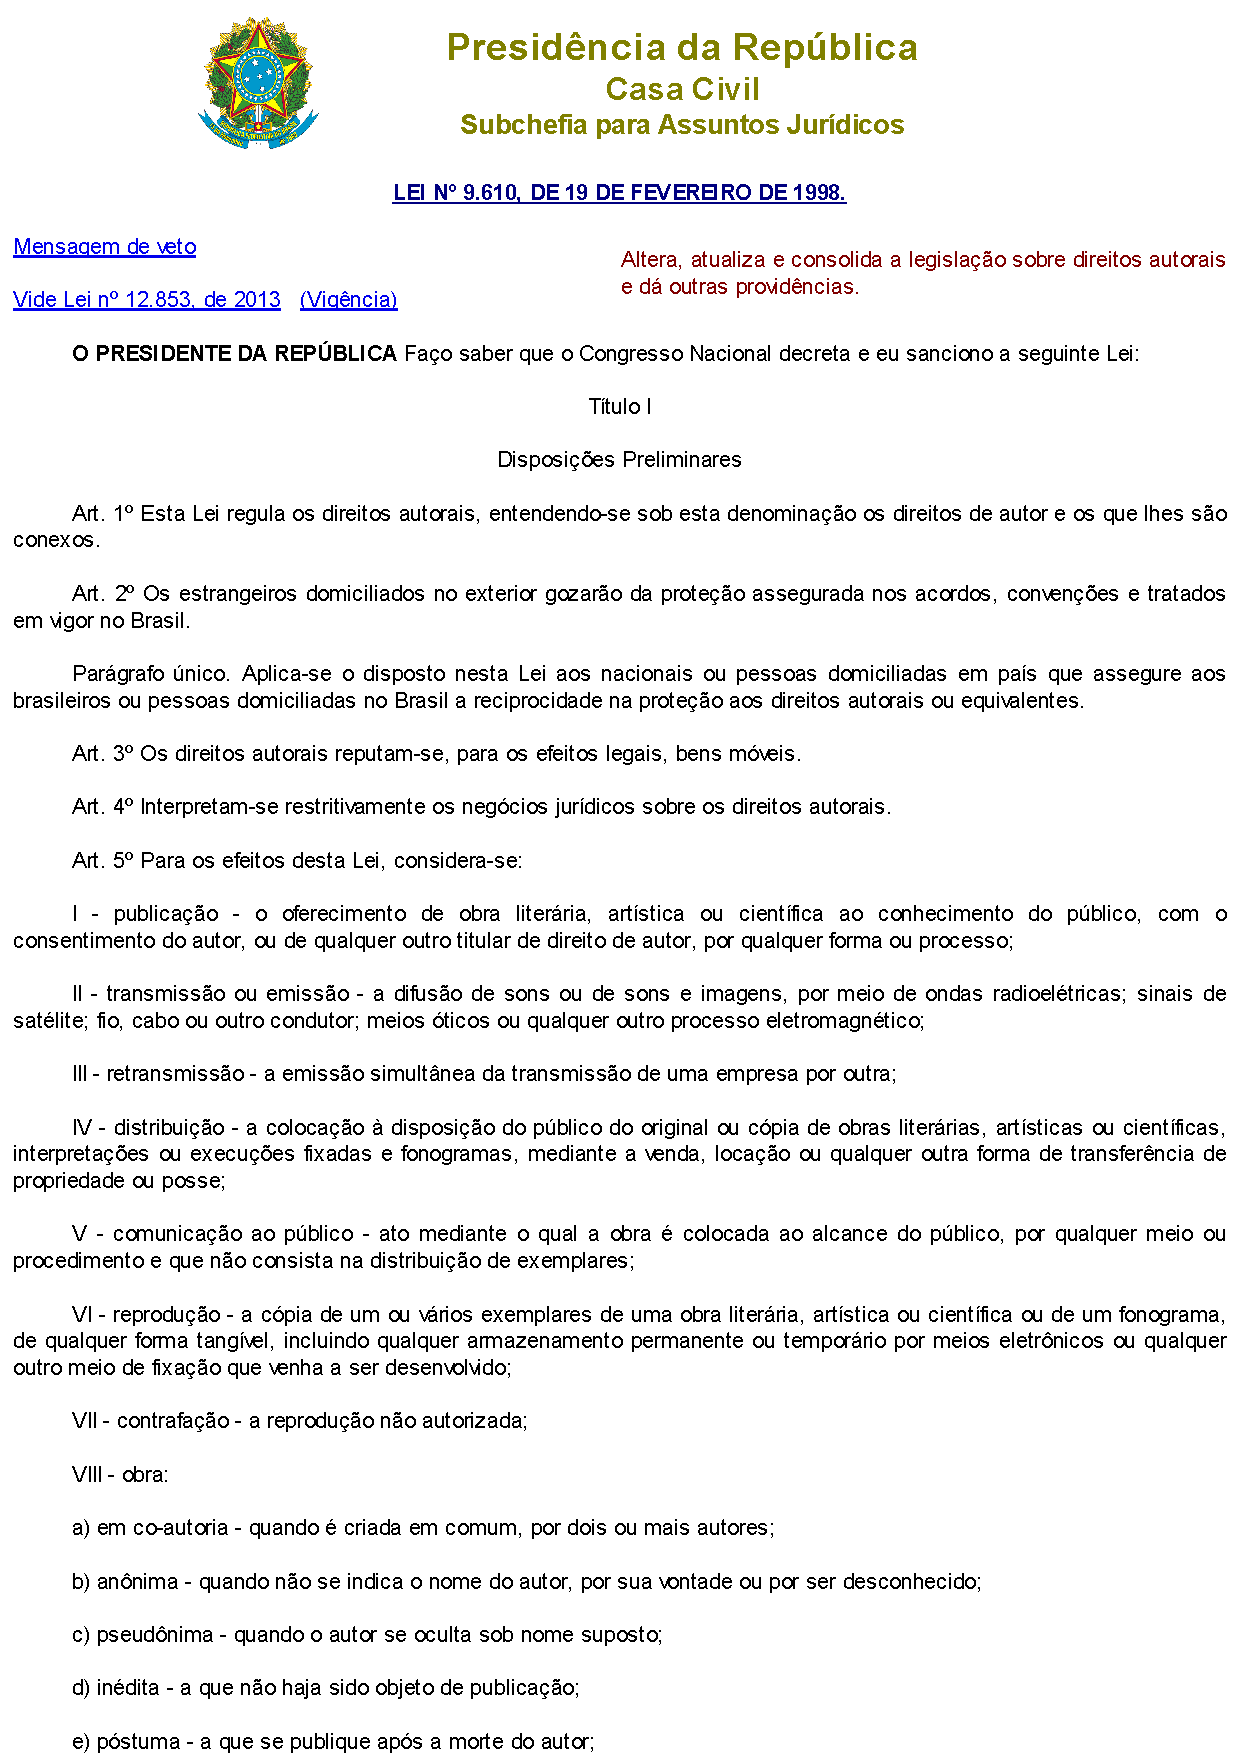
\includegraphics[width=\textwidth]{./PosTexto/Ilustracoes/lei-n9610-p1}}%% Imagem (Dimensões e localização)

\centerline{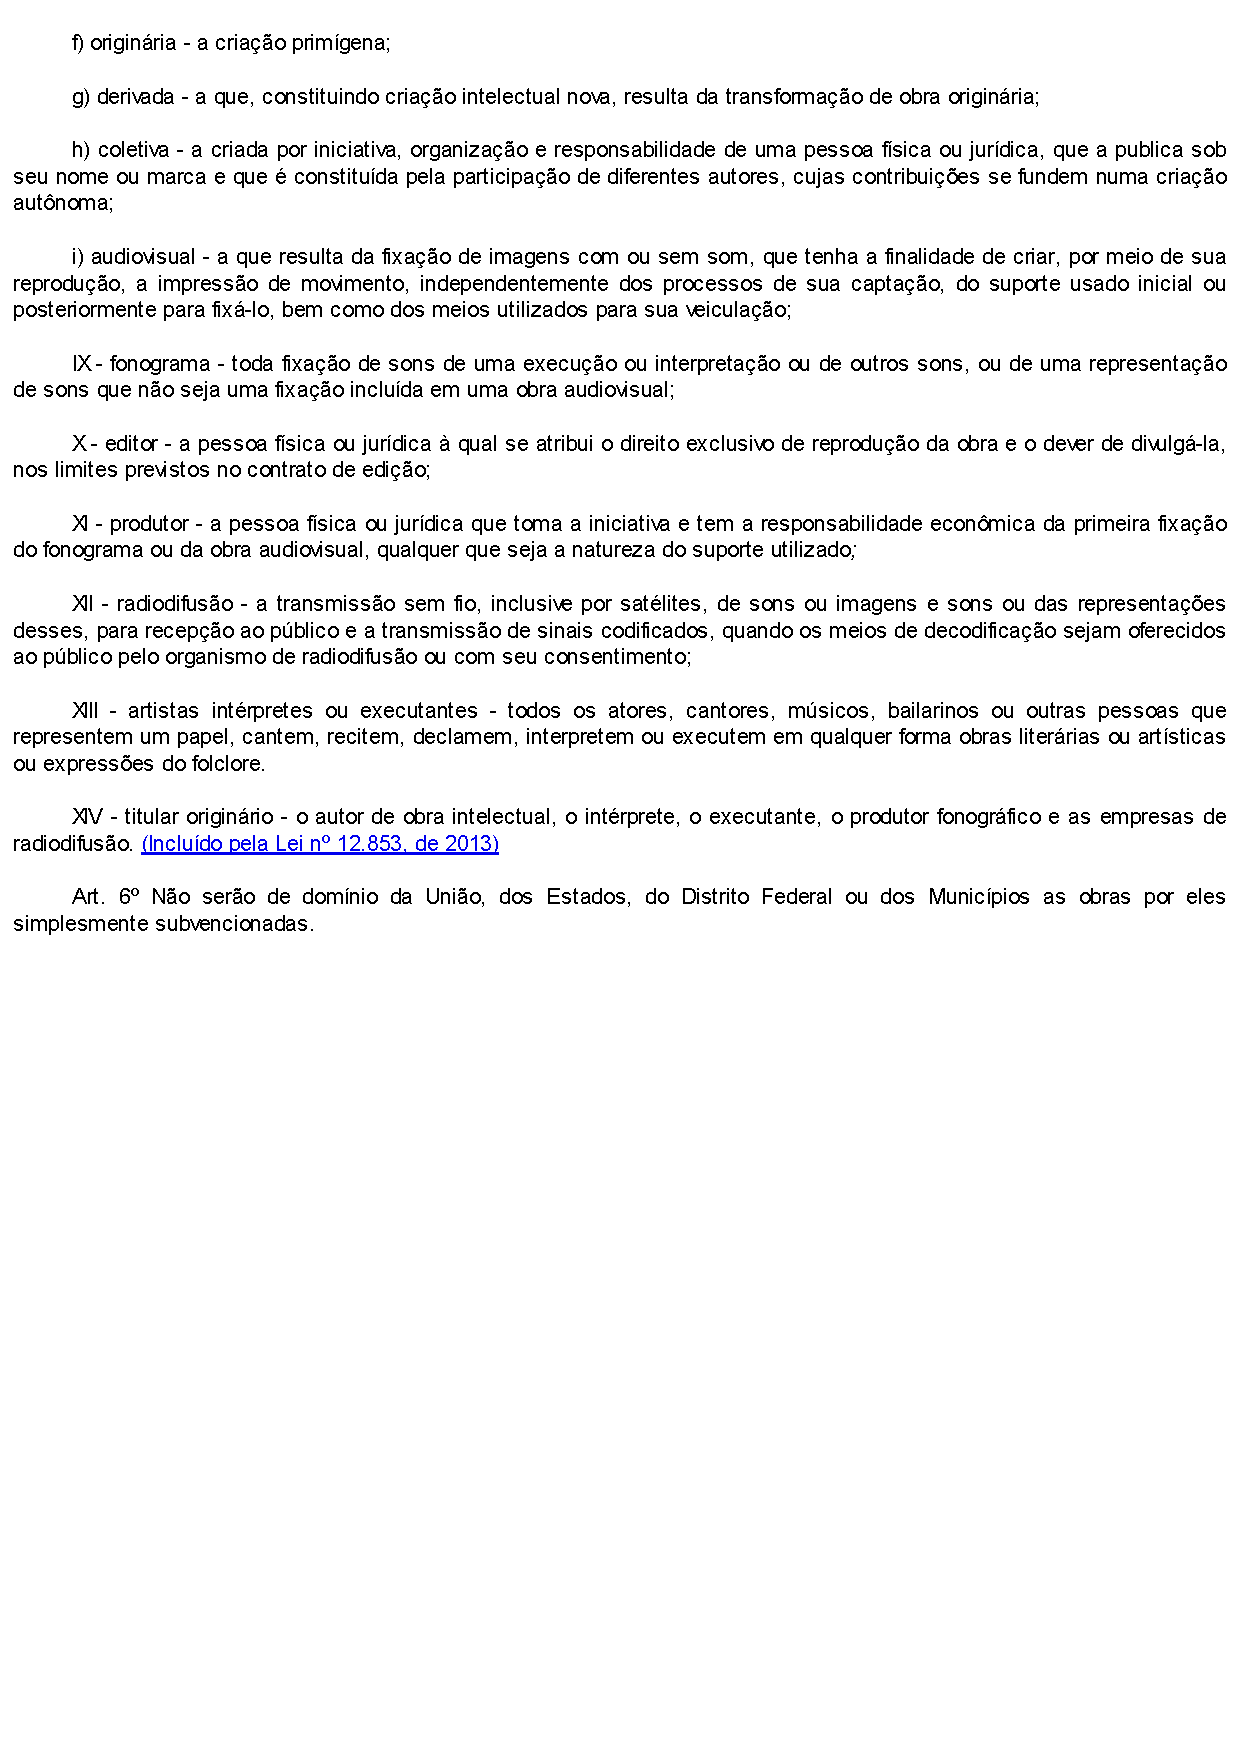
\includegraphics[width=\textwidth]{./PosTexto/Ilustracoes/lei-n9610-p2}}%% Imagem (Dimensões e localização)
%% Anexo - Comente para remover este item
  %%%% ANEXO B
%%
%% Texto ou documento não elaborado pelo autor, que serve de fundamentação, comprovação e ilustração.

%% Título e rótulo de anexo (rótulos não devem conter caracteres especiais, acentuados ou cedilha)
% \chapter{Normas para elaboração de trabalhos acadêmicos}\label{cap:anexob}%% Anexo - Comente para remover este item
\end{arquivosdeanexos}%% Não comente esta linha

%% Índice - Adiciona um índice remissivo.
%\incluirindice%% Comente para remover este item

%% Fim do documento
\end{document}%% Não comente esta linha
